\documentclass[man, floatsintext]{apa7}

\usepackage{lipsum}
\usepackage{tabularray}
\usepackage{multirow}
\usepackage[american]{babel}
\usepackage{subcaption} 

\usepackage{csquotes}
\usepackage[style=apa,backend=biber,doi=false,url=false]{biblatex}
\addbibresource{bibliography.bib}
\usepackage{float}
\usepackage{graphicx}
\usepackage{amsmath}
\usepackage{float}

\graphicspath{{./figures}}
\title{Modelling the effects of information gathering on social decision making}
\shorttitle{Modelling the effects of information gathering on social decision making}

\author{Damon Hayhurst}
\date{\today}

\makeatletter
\renewcommand{\maketitle}{
	\begin{titlepage}
		\centering
		\vspace*{0.4in}
		{\Huge \bfseries \@title \par}
		\vspace{0.2in}
		{\LARGE Damon Hayhurst \par}
		\vspace{0.3in}
		{\Large Project Report Submitted as\par}
		{\Large partial fulfilment for the\par}
		{\Large Degree of Cognition and Computation,\par}
		\vfill
		{\Large Birkbeck, University of London\par}
		{\Large \@date \par}
		\vfill
		{\Large
			\begin{center}
				I confirm that this write up is my own work and does not involve\par
				plagiarism as defined in the module information provided
			\end{center}
		}
		{\Large Signed and dated\par}
		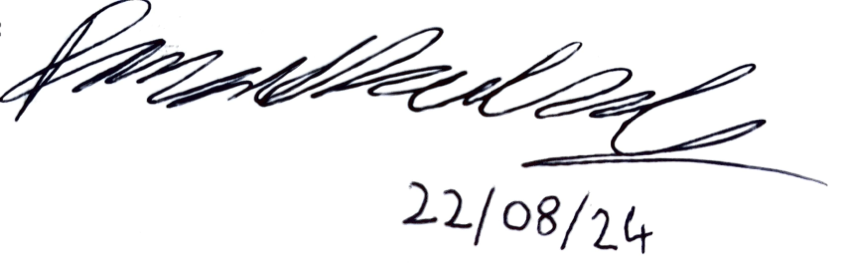
\includegraphics[width=0.5\linewidth]{figures/sig.png}
	\end{titlepage}
}
\makeatother

% Custom abstract environment to center the text
\renewenvironment{abstract}{
	\clearpage
	\null
	\vspace*{0.4in}
	\begin{center}
		 Are decisions made in our own self-interest influenced by the manner in which we form our conclusions? Using a modified version of the Message game, we looked at the way in which potential profits to self and losses to others modulated dishonest behaviour. In a secondary data analysis, we looked at whether individual differences in mouse tracking data could be used to predict dishonest choices. Using Dynamic Time Warping and heirarchical clustering, we found that process data from the trials could be clustered in to two groups revealing differing information gathering strategies. One group that characterises a more patient and comparative approach forgo small profits to themselves more to engage in altruistic behaviour. The other group share traits that could be defined in terms of sequential search with shorter dwell periods and show more of an aversion to lying when profits greater. Findings corroborate similar models found in non-social decision making contexts.
	\end{center}
	
	\vfill\null
	\clearpage
}

\begin{document}
\raggedbottom
\maketitle

% Project execution which includes: originality of ideas, independence, ability to act on advice and time and effort expended

\abstract

% Abstract which includes: completeness, clarity and succinctness


% Introduction which includes: breadth of the review, understanding of the literature, description of aims or hypotheses, organization and structure and clarity

% What is the breadth of the review?
% The review is about investigating the strategies employed when making decisions in a social context, using the messenger game as a framework within which to investigate such strategies. The breadth therefore comes from looking at investigations into the ways in which search strategies have been shown to influence decison making.
% Intertemporal Choice
% link between strategy and choice
% Bounded reality
% Process Tracing


%The background to the study should be provided here including a review of relevant literature and theory and clear statements about the aims and objectives of the study.




\section{Background}

\subsection{Understanding decision making in humans}

Present day understanding of decision making in humans takes it's inspiration from Herbert A Simon's approach of Bounded Rationality. Where prior understanding suggested that human beings act as  rational agents always seeking to maximise self interest. Bounded Rationality suggested that humans capability to act in a perfectly rational manner was constrained by internal and external factors.

%Herbert A Simon first outlined the idea that human behaviour in decision making was not to be defined by the decisions taken but that of the information surrounding the decision. This concept of 'Bounded Rationality' suggested an approach that took consideration of the contextual information regarding the decision as well as the computational capacities available to the decision maker. The concept sought to defy prior notions that human behaviour in decision making could be understood through a global notion of homo economius; Where decisions taken by agents were always perfectly rational, seeking to maximise their own self interests, and, instead, suggested that a human's capability to be perfectly rational was constrained by internal and external constraints.

Bounded Rationality places as much of an emphasis on the processing of information during the decision making as the decision itself. Pivotal to the concept, it was suggested that human's mental capacity to make choices is subject to heuristics or mental simplifications that contend with it's ability to be a perfectly rational agent but aid it's ability to make decisions in the face of increasing complexity (\cite{payneTaskComplexityContingent1976}).  Simon outlined Satisficing as a key mechanism employed in the face of decisional complexity. Such a model of process attempts to define the appropriate option amongst choices as being the first option to surpass a pre conceived threshold. Rather than cope with the cognitive overhead of comparing every option against all of the others in a perfectly rational manner, humans will opt for the first choice that is deemed sufficient and satisfactory (\cite{simonBehavioralModelRational1955},\citeyear{simonRationalChoiceStructure1956d}).

Early work into the mechanisms that perpetrate the notion of Bounded Rationality revealed the necessity for capturing process data. The Priority Heuristic attempted to explain choices within the context of simple monetary gambles using an ordered list of criteria. While the mechanism was shown to be significant at the aggregate level, the model failed to capture differences at the individual level. Further research into the manifestation of the Priority Heuristic, using process data, uncovered that in actual fact the underlying process did not mimic the priority ordering set out by the heuristic. The data, however, revealed that choice could be predicted significantly by the number of transitions into and out of a choice. The uncovering of such mechanisms highlights the need for processing data in explaining how humans make decisions. Process data can provide the explanatory power for decision making differences and inform the development of heuristics that can be applied at the individual level (\cite{brandstatterPriorityHeuristicMaking2006}), (\cite{willemsenVisitingDecisionFactory2011}).

\subsubsection{Decision making as a cognitive process}

The deliberation between two option does not represent two discrete states in cognition. Mental activity occurs throughout the decision making process. In this sense, cognition is best viewed as a continuous system with a set of intermediary states representing a graded spectrum between both options. The two classifications acting as attractor basins for which the decision making process finally rests in (\cite{spiveyContinuousDynamicsRealTime2006}).


%It is important to note that it is widely believed that human's decision making strategy is constructed contingent on the task demands and individual preferences. Decision making strategies have been shown to vary widely based on the number of choices at hand and the task complexity (\cite{payneWalkingScarecrowInformation2004}). Human's have a 'toolbox' of strategies which can be utilised in the cwhen it comes to information gathering and the choice reflects task demands and individual preferences. Such strat

\subsection{Capturing the decision making process}

Process tracing is a methodology used to gain insight into the decision-making process by extracting data that reveals the underlying cognitive mechanisms. This involves various techniques, ranging from simple verbal protocol analysis, where participants articulate their thoughts aloud, to advanced methods like neural tracing using MRI machines (\cite{fordProcessTracingMethods1989}). The goal of these methods is to capture detailed data from different stages of the decision-making process and use that information to inform and develop process models.
	

Studying decision-making involves analysing different stages, such as problem identification, information gathering and decision selection. Each stage requires specific methods of data extraction to effectively capture the nuances of decision-making. For instance, in the information gathering stage, researchers might employ eye-tracking to see where attention is focused, or they might use tools like MouseLabWeb to observe how individuals search for and process information. The choice of instrumentation is crucial, as insights into decision making are limited by the resolution and representation of the output data. Efforts must be made to consolidate these representations with process models in order to enhance their development and applicability.

\subsubsection{MouseLabWeb}

MouseLabWeb (and offline counterpart, MouseLab) is one such development in process tracing that fosters an environment fit for observing the information gathering stage in decision making. Utilising the dynamic properties of Javascript in the context of a web page, MouseLabWeb describes an interactive framework that tracks users' attentional focus on decision-making elements as they engage with different options. MouseLabWeb experiments consist of a browser page containing adjacent pairs of hidden view boxes. Each pair represents an option and the make up of each pair is a  box containing a piece of information relevant to that particular option. Positioning the mouse cursor over one of these boxes reveals the concealed information. The mouse cursor movements are tracked and then stored on a trial by trial basis. Such data can be used to observe where a participant's focus lies. The simplistic design of a MouseLab experiment reduces the cognitive load on the participant, affording them simple cursor movements instead of lookup to memory (\cite{MouselabWEBa}). 

\subsection{Interpreting information gathering data}

Interpreting results from a MouseLab experiment involves discerning attributional qualities from a given trace. \citeauthor{costa-gomesCognitionBehaviorNormalForm2001} define two events in a process trace that can provide insight into the underlying characteristics of a trace. Occurrence, being that a particular piece of information has occurred within a process trace and therefore, that piece of information can be considered as part of the overall strategy underlying the trace. An absence of an occurrence of a particular piece of information suggests a strategy that is made without considering the full picture and could be conceived as impulsive. And Adjacency, if two adjacent pieces of information occur sequentially within a trace then it means a comparison has likely to have taken place. An absence of adjacency could represent a disregard for certain aspects underlying the decision such as in social preference based choices, where the adjacent pairs show to be payoffs related to you or the other participant. An absence of adjacency in this case suggests motives that are wholly self concerned. The decisional lookups and their contextual information can together help attach a type to a specific process trace (\cite{costa-gomesCognitionBehaviorNormalForm2001}).

\citeauthor{reeckSearchPredictsChanges2017b} found success through observing both the acquisition of information and the duration within which they looked at said pieces of information. Using the Intertemporal Choice task as options in the MouseLab experiment, they were able to disseminate two underlying search strategies and showed success in linking their use to the decisional outcome. Using K-means clustering, two types of strategy emerged. Comparative searchers, who exhibited a more patient approach involving large proportions of adjacency and integrative searchers who showed fewer occurrences of each piece of information and shorter durations of observation in their process trace before deciding. Success was found in observing that comparative searchers were significantly more likely to pick the more patent option in the Intertemporal choice task (\cite{reeckSearchPredictsChanges2017b}). 


\subsection{The neurobiology of social decision making}


Evidence suggests that neural circuitry involved in social decision making does not distinguish itself from that of the circuitry involved in other forms of  decision making. Value based processing found in ventromedial prefrontal cortex (vmPFC) supposedly integrates signals from other areas of the brain during the decision making process, feeding signals back based on value representation change. This understanding, known as the extended common currency schema, directly contrasts prior theories that suggested our social decision making skills evolved as part of a separate adaptive system (\cite{ruffNeurobiologyRewardsValues2014}).

The specificity in social decision making comes from the neural circuits that the vmPFC tracks during social dilemma is faced. The lateral prefrontal cortex (LPFC) which tracks value to self and the right temporoparietal junction (rTPJ) which tracks value to others. It was suggested that these two circuits were involved in the social decision making process within a study that used the Message Game (further elaborated upon in the Methods section) as it's stimuli. Using neuroimaging technology, \citeauthor{shusterContributionSelfOtherregarding2020} observed the two neural circuits independently tracking their respective motives by modifying trial parameters specific to the Message game that altered the perceived social outcomes. The vmPFC representing the value computation between the two varied on an individual level (\cite{shusterContributionSelfOtherregarding2020}).

\section{Aims}

The aims of this study is to gain an insight into how the effects of information gathering influence our decision making in a pro-social context.  Using process tracing, we hope to observe and characterise strategies that are utilised in order to arrive at these decisions. Such an approach hopes to shed light further on the processes that underlie decision making in human behaviour.

In this study, we hypothesise that there are individual differences between information gathering strategies and that strategy can be used as a predictor in social decision making. By exploring the relationship between task condition and information gathering strategy we look at whether differences in own profit's and other's losses, which have previously shown to alter likelihood of lie, contribute to alterations in strategy. And, using clustering techniques, we look across the whole population of trials to see whether differences in strategy reveal. Finally, we ask to what extent differences in strategy drive dishonest behaviour in social contexts.

\section{Methods}

% Methods which includes: completeness, justification of choices/decisions made, organization and structure, clarity, reference to ethics

% This section is composed of several sub-sections and should give sufficient information to enable the reader to know exactly what was done:
%
%Participants (in projects using human participants).This will be skipped if you are not using human participants. Please specify in this section that ethical approval was obtained and include the ethics approval number and the title of the ethics application.
%
%Materials and Stimuli (all stimuli involved in your project, including software, questionnaires, programmes, interview schedules, for example). Feel free to include pictures of your stimuli. Describe everything.
%
%Design and Procedure (this section should be detailed enough that someone not familiar with your project should be able to run it themselves/understand how you recruited participants, collected data and so on). 

A secondary analysis was carried out from the results of pre existing experiment. The primary stimuli, of which, was a variation of The Message Game that was carried out within a MouseLabWeb environment. 

\subsection{The Message Game}

The Message Game is a form of experimental game that models a particular complexity faced by individuals in pro-social environments. The game uses honesty to illustrate how decision making can be affected by value judgements that pit our own self interest against our altruistic sensitivities. 
The game involves two roles. The Sender and the Receiver. The Sender must send a message to the Receiver informing them of a particular box to open from a choice of four. Each of the boxes contains differing amounts of money for the Sender and the Receiver should that box be chosen. The Sender can ultimately see what's inside each of the boxes in terms of how much money they will receive versus the amount that the Receiver will. Only the Receiver opens the box, however. A message is sent by the Sender to the Receiver with words to the affect of 'Box X is best for you'. The dishonesty comes from the Sender being able to suggest a box that might not necessarily represent the truth and instead picking a box that contains a larger amount of money for themselves and less money for the Receiver. With the Receiver unable to see the quantity of money they potentially missed, they must decide whether to trust the Sender's recommendation and open the suggested box.

\subsubsection{Experimental Variation}

In this variation, focus is placed entirely on the Sender. Two of the boxes are blank meaning that the Receiver has no choice but to pick the Sender's recommendation or risk a 2 in 3 chance of getting no monetary income. The participant plays as the Sender for the majority, however, does get to have a go at playing at the Receiver to understand the dilemma faced. The participant then spends 80 trials in the Sender role where the process data is tracked. The position of the monetary rewards in the boxes are then altered on a trial by trial basis so that decisions are encouraged to be deliberate and do not succumb to laziness. 

The values held in each of the two boxes vary on a trial by trial basis. Each of the two boxes consists of two values representing a profit for the Sender and Receiver. These boxes always contain differing amounts for the Receiver and Sender. The box with the higher amount for the Receiver, if chosen, represents the Sender telling the truth to the Receiver. Likewise, the box with the lower amount represents the Sender making a dishonest claim to the Receiver.

\begin{figure}[H]
	\centering
	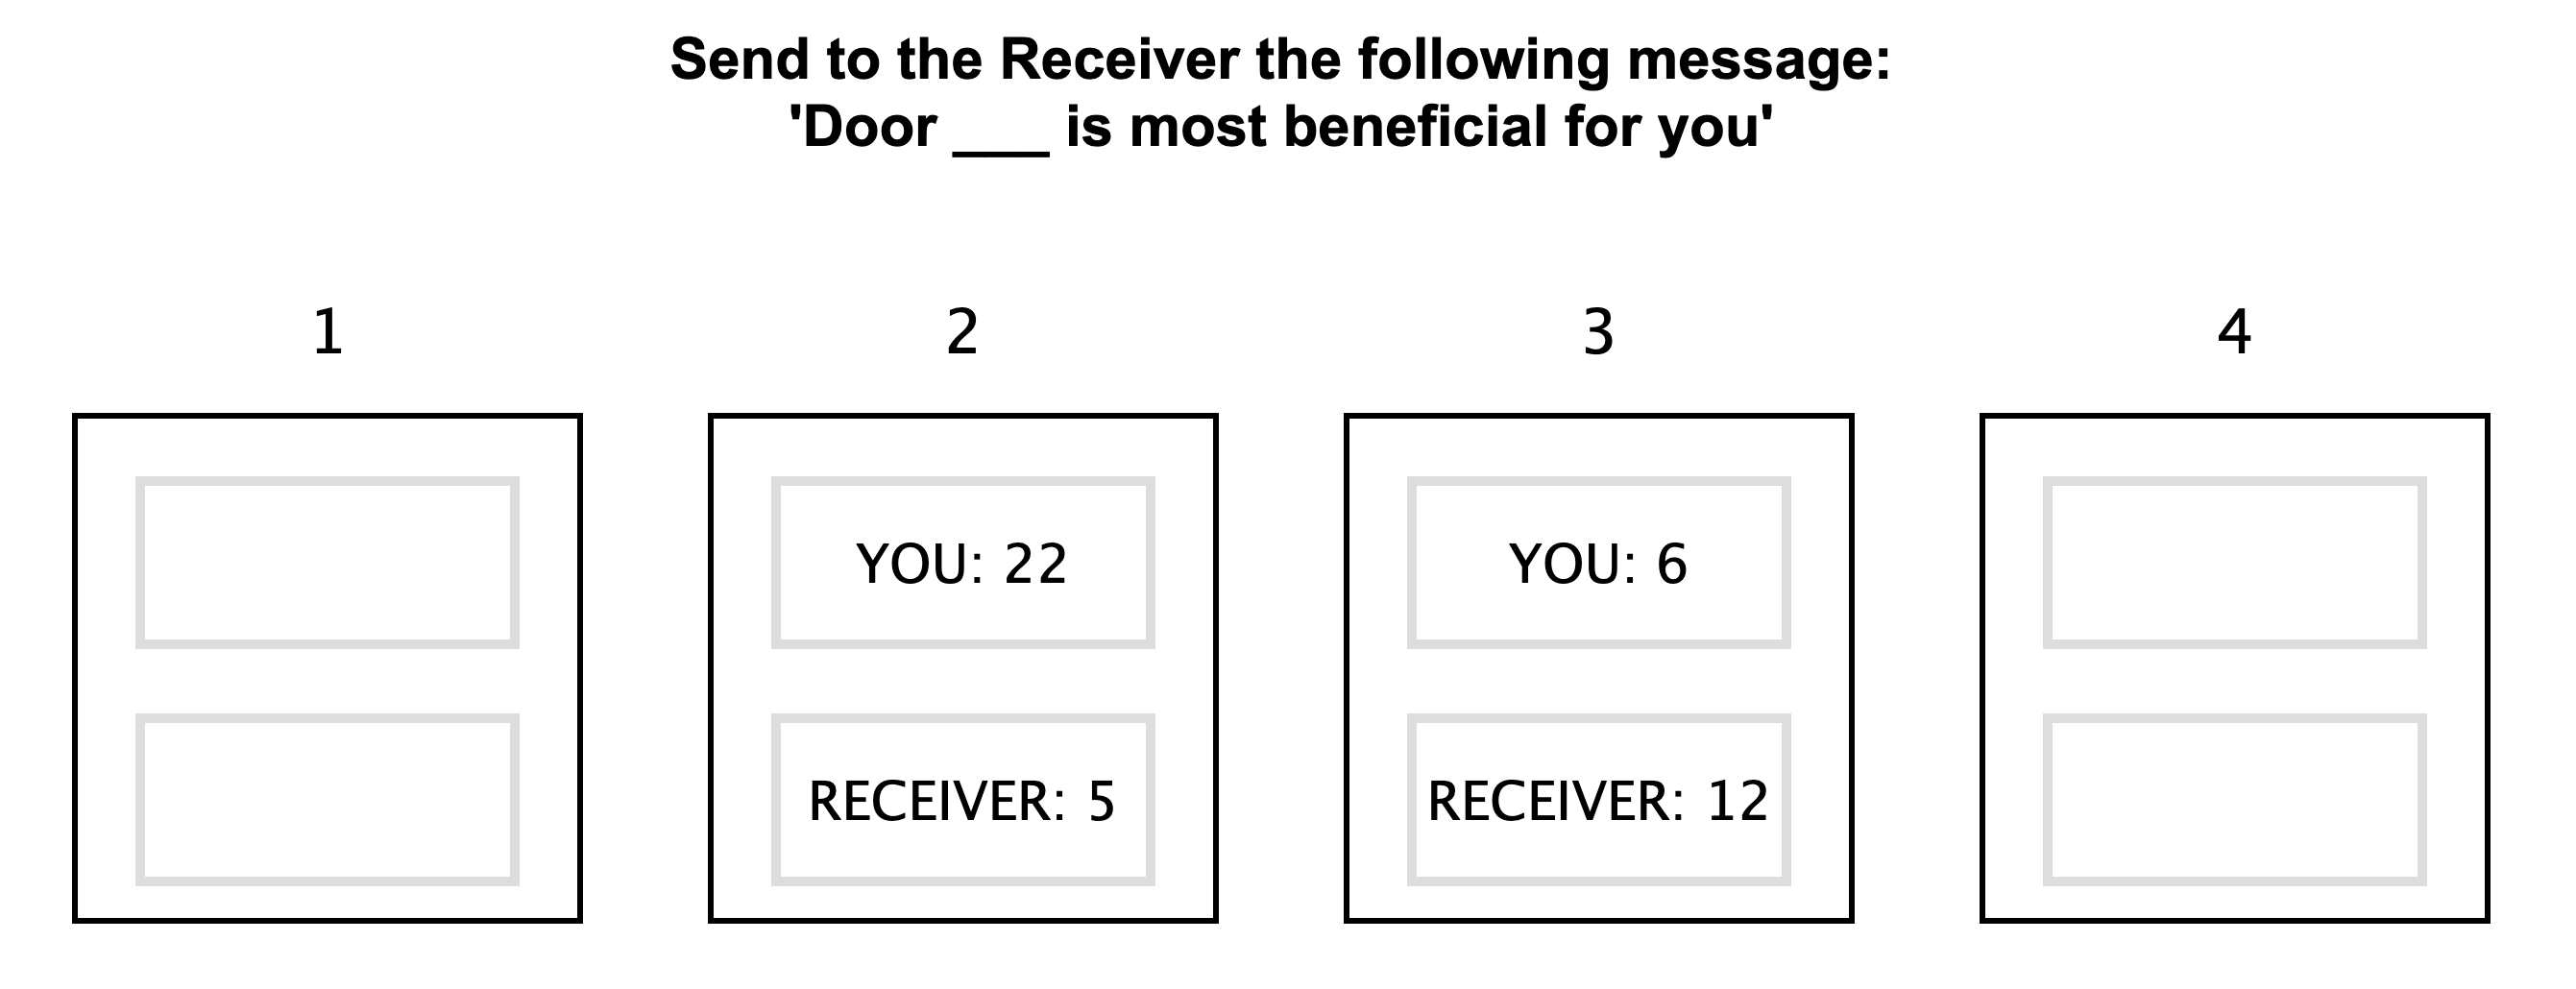
\includegraphics[width=0.75\linewidth]{figures/NOT HIDDEN.png}
	%\figurenote{This is a great figure.}
	\label{fig:AOIs}
	\caption{Layout of boxes and AOIs for one specific trial. Door 2 represents the Sender choosing to lie. Door 3 represents the truth. The 2 AOIs inside door 2 are SELF LIE (top) and OTHER LIE (bottom). Door 3 hold the AOIs, SELF TRUE (top) and OTHER TRUTH (bottom).}
\end{figure}


Being that the trials were carried out in a MouseLabWeb environment, the amounts contained within the boxes shall be referred to as Areas of Interest (AOIs). The AOI representing what amount the Sender receives for the truth telling box is SELF TRUE and the one representing the amount for the Receiver is OTHER TRUTH. AOIs corresponding to the amounts for the dishonest box are SELF LIE for what the Sender receives and OTHER LIE for the receiver. Theses AOIs are the pieces of information hidden from view that can only be revealed by hovering a mouse cursor over the panel. Horizontally adjacent lookups correspond to comparisons of amount awarded to one particular role and vertical adjacency compares values awarded for both roles for a given option. The vertical order of the AOIs swaps as well in order to encourage deliberate observations.

\begin{figure}[H]
	\centering
	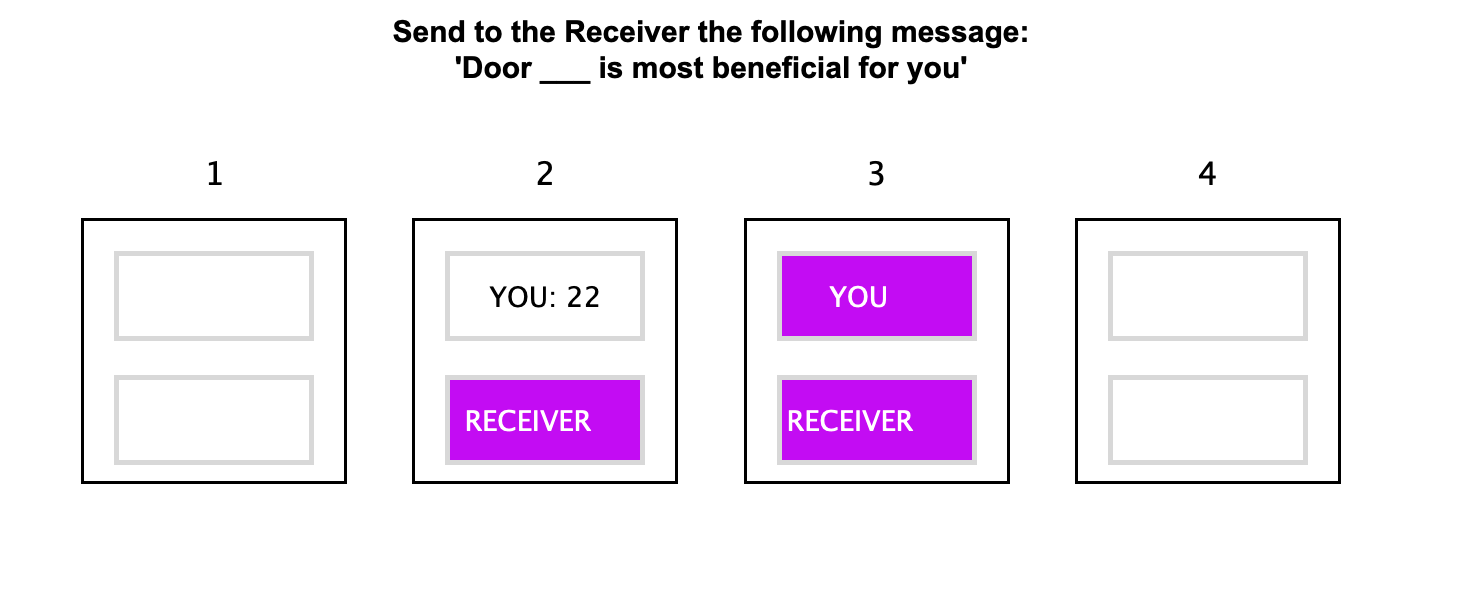
\includegraphics[width=0.75\linewidth]{figures/HIDDEN.png}
	%\figurenote{This is a great figure.}
	\label{fig:HiddenAOIs}
	\caption{What the participant sees during experimental trials. The top AOI of door 2 is currently being hovered over with the mouse.}
\end{figure}

With the values and positioning of each AOI altering on a trial basis, one can gain an insight into the process and circumstances that inhibit a participant from acting in a rational manner. The game theoretic viewpoint suggests that the Sender should always choose to act in their own self interest by picking the option that represents the maximum utility to themselves ie. the box with the most value to them. Ultimately there are no repercussions for lying and therefore rational agents only need to seek value from profit. Using human participants and recording process data, we can observe when a humans' s show aversion to self interest and their altruistic sensitivities take over.

\subsection{Procedure}

Results for the experiment carried out using the primary stimuli, the variation of the Message game, recorded a collective total of 89 participants. Rows represented a single trial for each participant. The rows provided information such as the values that were in each AOI, the selected box number, reaction time and a process trace.

Since trial order was randomised, an index number was assigned to each trial. That number was based upon every unique set of values contained within the AOIs. Trials that shared the same amounts were assigned the same index value. See Figure \ref{fig:Gains} and \ref{fig:Losses}. The trials could then be aggregated across participants based on the profits and losses earned by the Sender and Receiver per trial.

The trials were then grouped per participant and were assessed under a set of criteria that might warrant their exclusion. A breakdown of these can be found in the Results section.

Each remaining trial had a process trace consisting of a semi-colon delimited set of timestamps and coordinates representing the position of the mouse cursor at any given time during the trial.  By corroborating this information with the stated participants screen width and the per trial position of each box and containing values, it could be calculated whether a particular timestamp represented a cursor position that was inside one of the four AOIs. From this, a timeline could be built showing durational occurrences of any of the four AOIs within the process trace.

\subsection{Average Analysis}

Using the newly created timeline, the average dwell for each of the four AOIs was calculated per trial. Along with the number of transitions between adjacent AOIs per trial. 

\subsection{Cluster Analysis}

The timelines were assessed under a further notion of similarity. By taking into account a point by point comparison between each of the timelines on the millisecond level, underlying trends can be uncovered that forgo the detection of average calculation. The consolidation of such point data provides the affordance of perceiving time series similarity under a single distance measure. This output can then be used to inform the formation of clusters and classification.

\subsubsection{Dynamic Time Warping}

Dynamic Time Warping (DTW) is a length-invariant measure of distance between two time series. It takes the minimum cost alignment between two sequences using a one to many comparison of each point. Where the Euclidean measure only takes into account a point to point mapping using equal length time series, the DTW measure doesn't abide by such strictness in it's comparison. Using a many to many approach means that a DTW measure can factor in patterns of activity that are approximate in both series and realise they're similarity. In this way, DTW can perceive relationships in time series that are shifted and subject to noise.

A pairwise comparison was drawn between each individual trial for each participant using  DTW as a measure of similarity. Each trial's timeline was represented in a n x 4 array where n was the quantity of milliseconds in the trial and 4 elements representing the binary state of each AOI describing whether the cursor was within it's bounds or not. Prior to comparison, each time series was subject to z normalisation. Thus, ensuring that greater variation in longer length series was accounted for and comparison could focus on the shape of the data.

\subsubsection{Clustering}

Hierarchical clustering was then used with the calculated DTW metric to achieve a desired number of clusters. The clustering mechanism used in this instance, Agglomerative, recursively merges clusters using a bottom up approach. Each cluster represents a single trial at the beginning and then trials are merged based on the comparison that represents the smallest distance. Clusters are then recursively merged with a cluster's proximity to another cluster being defined by the maximum distance that can be described based on the cluster's constituent trials. The process repeats until the number of desired clusters is reached.

In the analysis, the desired number of clusters was defined as the number that returned the highest value from the pseudo F statistic. The statistic identifies well-fitting clusters by maximising between-cluster variance while minimising within-cluster variance. By evaluating this measure up to 20 clusters, the resulting clusters were expected to represent a level of classification that avoids overfitting.



\section{Results/Findings}

\subsection{Trial and Participant Quantities}
\label{subsec:quantities}
The processing of data removed a proportion based on criteria that represented a lack of engagement with the experiment. Six participants were removed for not finishing it. 20 were removed for telling the truth over 95\% the time and a further 14 participants were removed for recommending the blank boxes to the receiver in over five percent of the trials.  Interestingly, no participants were removed for lying over 95\% of the time; despite this being the approach favoured in game theory.  A further 40 trials were removed from the dataset because they recorded decision making times that were three standard deviations away from the mean. An approach also taken by \citeauthor{reeckSearchPredictsChanges2017b}, suggesting a similar lack of engagement with the task at hand.

Irregularities and missing data that represented a failure in process tracing were also removed from the dataset. 10 participants were removed for having not recorded mouse coordinates in over 85\% of their trials and a further 108 trials removed from the remaining valid set because of similar lack of mouse coordinates. Irregularities in some of the coordinate data meant that AOIs could not identified through measurement. 42 trials were removed because of this and one participant also, that failed to record screen width data. If such impairments in the dataset had been included by merely estimating their missing qualities, it would have compromised the overall integrity. Omitting them highlights the essential role of accurate process tracing.

In further regards to accurate process tracing, some consideration was taken towards events that lasted under a threshold of 200ms. This process accounts for jittery movements by the participant and periods of dwell that do not amount to the recognised minimum for reading hidden text in object recognition (\cite{dicarloHowDoesBrain2012}) and MouseLab literature (\cite{willemsenVisitingDecisionFactory2011}). Once all events in each trial accounted for this threshold, a further 103 trials were removed from the total citing an absence of any remaining valid dwell events within AOIs. 

After accounting for engagement criteria and irregularities, the number of valid trials was recorded for each participant and a further six participants were excluded from the analysis. The number of valid trials for each of these participants represented a quantity that was less than three quarters of the intended 80 trials for each participant. Given, the ordering of each trial was randomised, the set of valid trials for each of these participants could represent biases in likelihood to lie relative to the whole data set.

From the original pool of 89 participants, only 32 remained after all removals. An overall data set that contained 2489 trial instances each with a valid process trace.

\begin{figure}[H]
	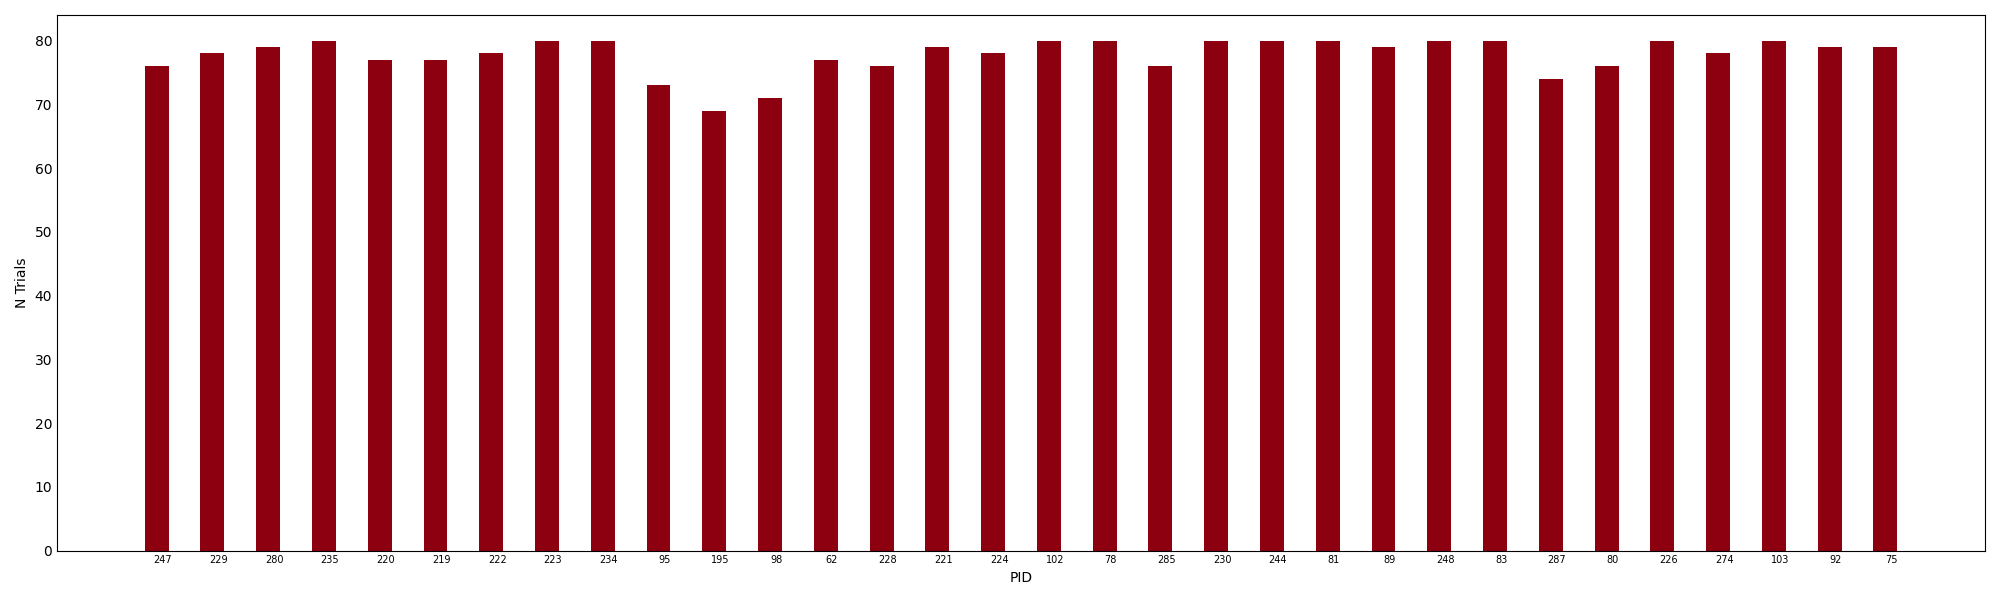
\includegraphics[width=\linewidth]{../plots/RESPONSE/NTrialsByPID.png}
	%\figurenote{This is a great figure.}
	\label{fig:NTrialsByPID}
	\caption{Bar graph representing number of trials in the final valid data set for each participant.}
\end{figure}

\subsection{Descriptives}

\subsubsection{Lie Percentage}

Across trials the propensity to lie displayed a high degree of variance. The average likelihood to lie on any given trial was 38\% $(N = 2489)$. Across participants, the propensity to lie was measured with a 22\% (Q1) - 51\% (Q3) interquartile range for a given individual. Across instances of unique trial, where unique is defined by the specific quantities pertained to in the boxes, the range was 0 - 90\% with an interquartile range of 16\% (Q1) - 59\% (Q3) for any given trial.

\begin{figure}[H]
	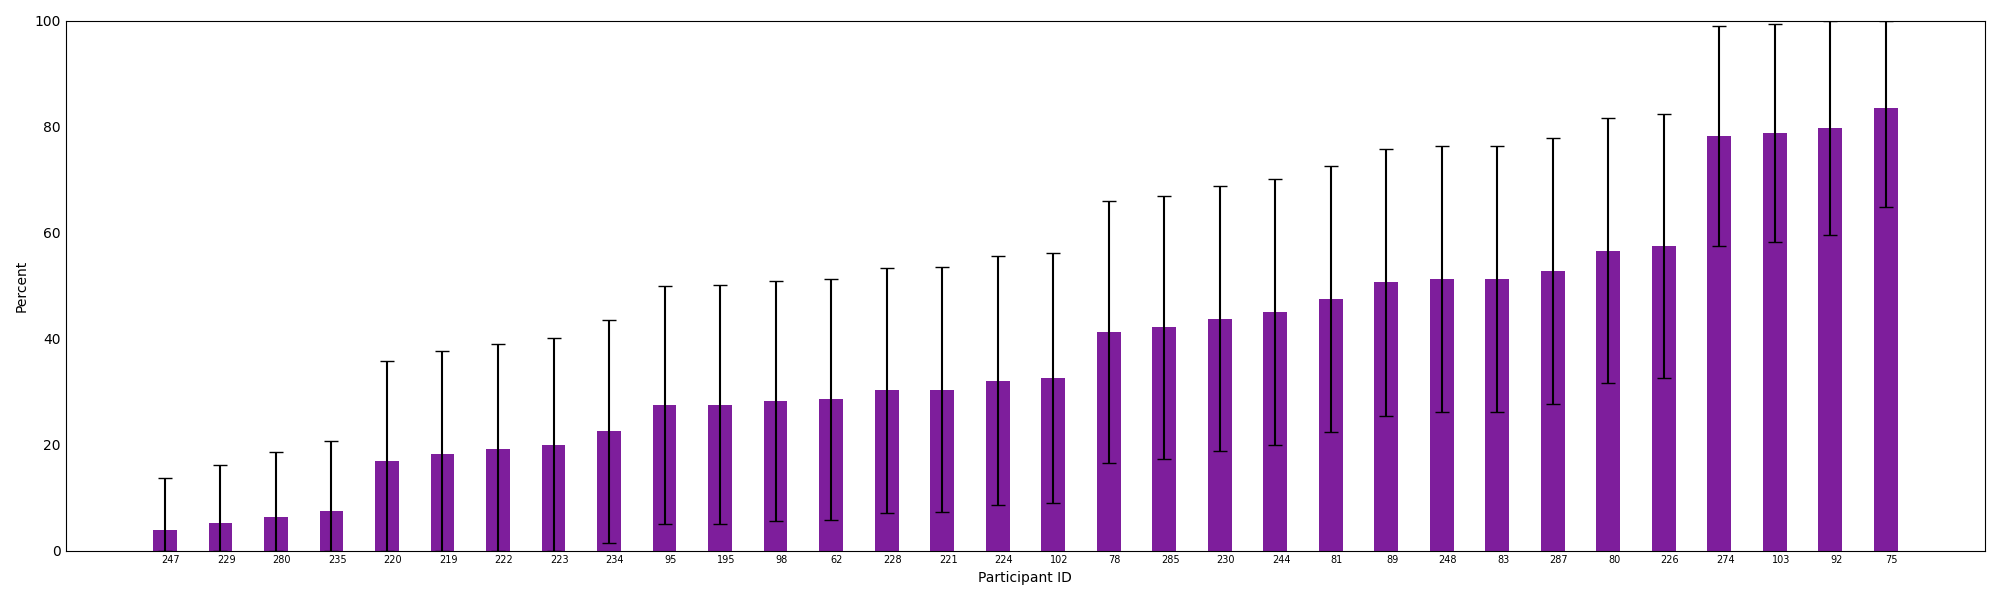
\includegraphics[width=\linewidth]{../plots/RESPONSE/PIDPercentLiesPlot.png}
	%\figurenote{This is a great figure.}
	\label{fig:PIDPercentLiesPlot}
	\caption{The percentage proportion of lie options chosen across participants}
\end{figure}

\begin{figure}[H]
	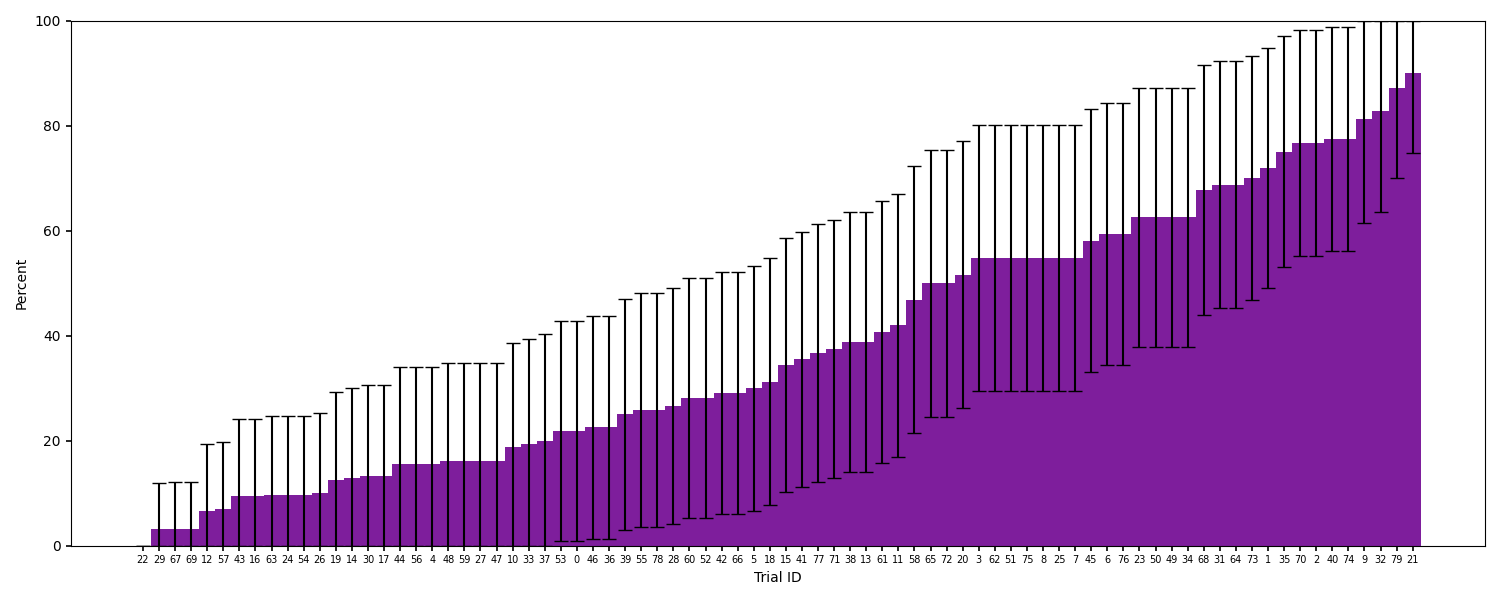
\includegraphics[width=\linewidth]{../plots/RESPONSE/TRIALIDPercentLies.png}
	%\figurenote{This is a great figure.}
	\label{fig:TRIALIDPercentLies}
	\caption{The percentage of lies per trial. Trial ID delineates each set of values that make up the condition of a trial ie. the values found in each of the AOIs. The set of 80 trial conditions were randomised for each participant.}
\end{figure}

\subsubsection{Dwell Time Distribution}

Reaction time (or the time it takes to make a decision) showed a large amount of range. The average reaction time was 6513 ms $(SD = 3050$ms$)$ with an interquartile range of 4393 (Q1) - 7871 ms (Q3).

The amount of time spent dwelling on one of the four AOIs on the screen was observed. The AOIs, SELF LIE ($M = 470$ms, $SD = 428$ms), SELF TRUE ($M = 420$ms, $SD = 343$ms), OTHER LIE ($M = 571$ms, $SD = 423$ms) and OTHER TRUTH ($M = 604$ms, $SD = 472$ms) all recorded means within 150ms of one another. 

\begin{figure}[H]
	\centering
	\caption{Distribution of number of transitions between AOIs across trials.}
	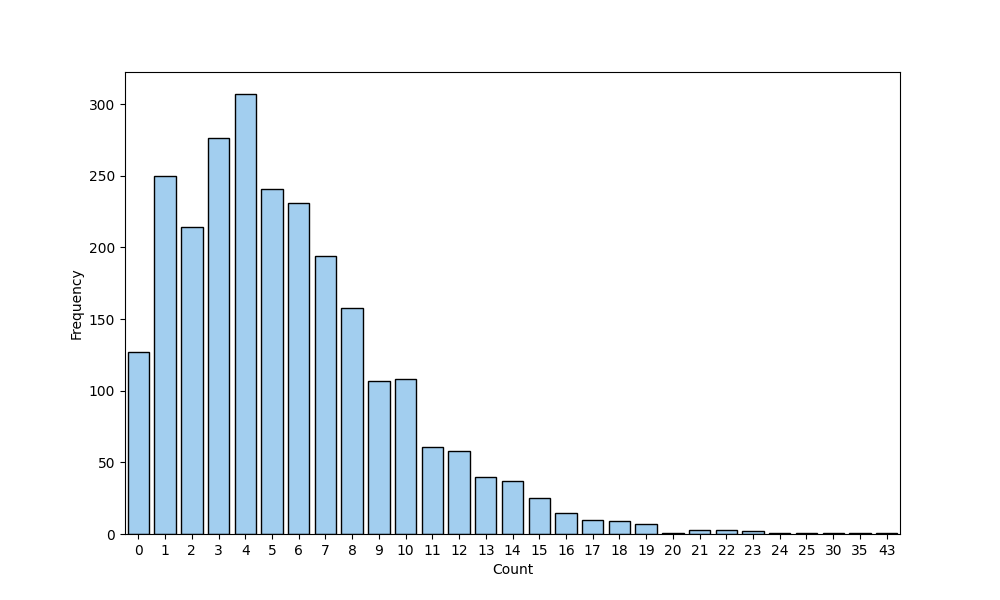
\includegraphics[width=0.65\linewidth]{../plots/Dwell/N_TransitionsDistPlot.png}
	%\figurenote{This is a great figure.}
	\label{fig:NTransitionsDistPlot}
\end{figure}

The number of transitions is marked by where a participant would move the cursor from one AOI to another was also observed across all trials. The mean number of transitions between AOIs was ($M = 5.6$, $SD = 4.1$) with an interquartile range of 3 (Q1) - 8 (Q3).

\subsubsection{Trial Condition}

\begin{figure}[H]
	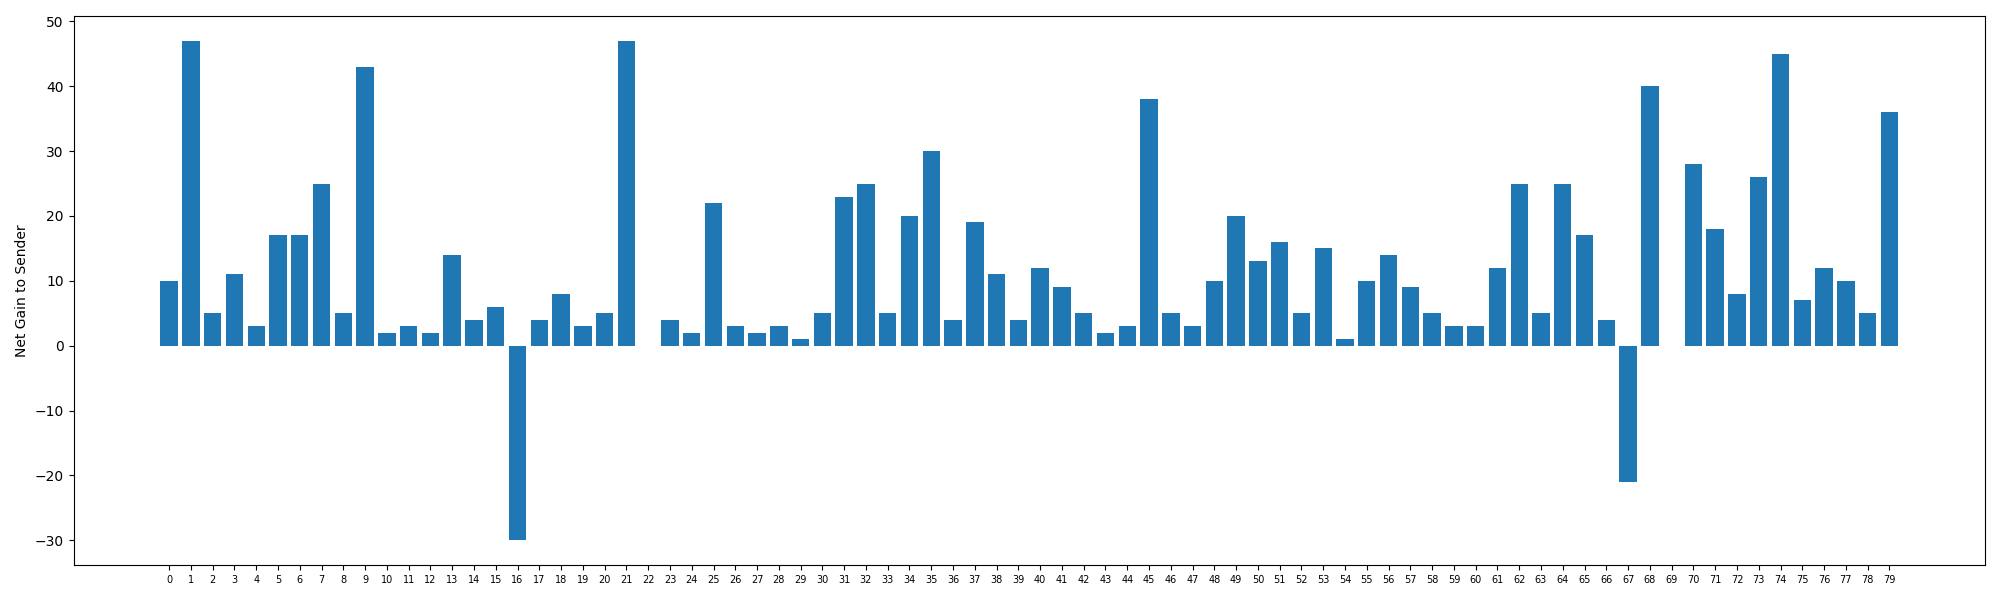
\includegraphics[width=\linewidth]{../plots/TrialIndex/Gains.png}
	\caption{Bar chart showing the amount gained by the Sender should they choose to lie in the corresponding trial.}
	%\figurenote{This is a great figure.}
	\label{fig:Gains}
\end{figure}

Each of the trials involved giving differing amounts to the sender and the receiver based on whether the Sender decided to lie or not. The average net gain to the sender was 12 $(SD = 13)$ per trial. The median was 8 and had an interquartile range of 4 (Q1) - 17 (Q3). The average loss to the receiver was 11 $(SD = 9)$ with a median of 8 and an interquartile range of 4 (Q1) - 15 (Q3).

\begin{figure}[H]
	\caption{Bar chart showing the amount lost by the Receiver should the Sender choose to lie in the corresponding trial.}
	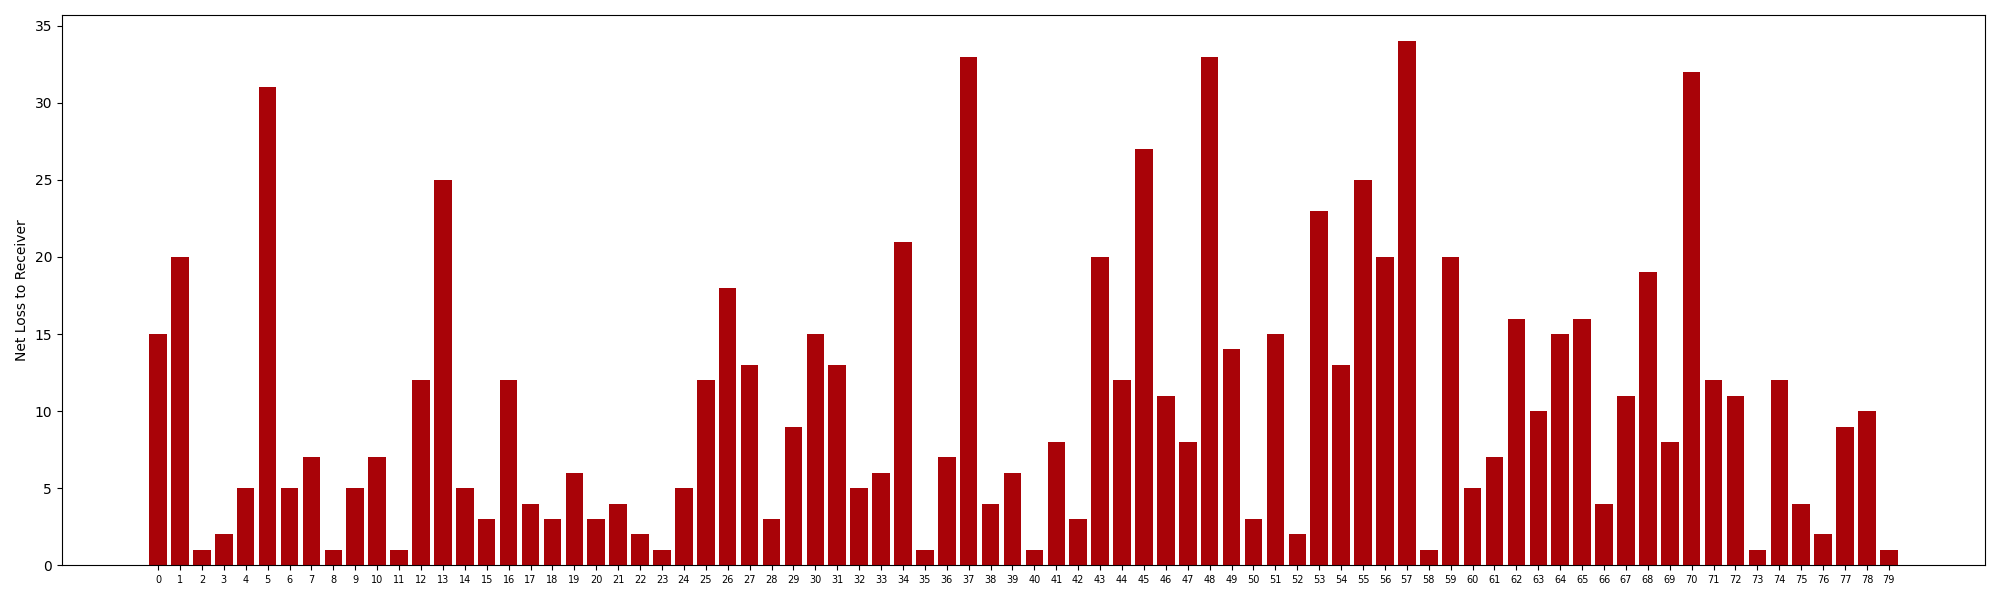
\includegraphics[width=\linewidth]{../plots/TrialIndex/Losses.png}
	%\figurenote{This is a great figure.}
	\label{fig:Losses}
\end{figure}

\subsubsection{Lie proportion by trial condition}

The percentage that chose to lie in the experiment increased as the net gain to the Sender did.  Senders lied the least when they incurred a net loss by lying. Only choosing to lie 6\% $(N = 63)$ of the time. From net gains below 10 to above 10 the percentage who chose to lie increased, from 24\% $(N = 1336)$ to 55\% $(N = 1153)$. When gains were above 20, the percentage who chose to lie in this task scenario grew to 70\% $(N = 560)$ and when they were above 30 the amount who decided to lie showed further increase but to a lesser extent 76\% $(N = 250)$.

\begin{figure}[H]
	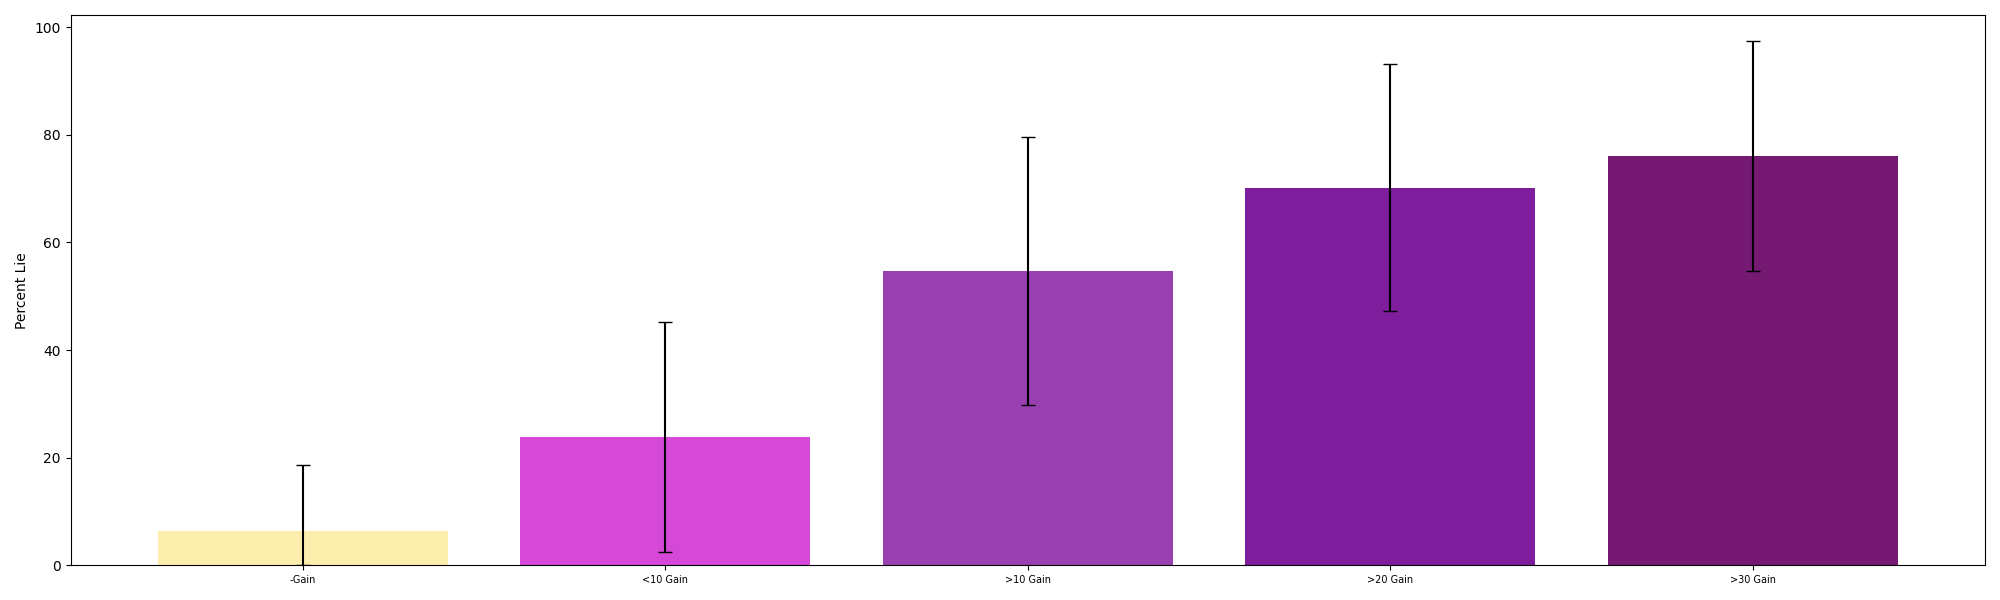
\includegraphics[width=\linewidth]{../plots/RESPONSE/NetGainLie.png}
	\caption{Percentage who chose to lie based on the amount gained by lying.}
	%	\figurenote{+10 gain represents the proportion who chose to lie for all amounts above 10 and also applies for +20 and +30.}
	\label{fig:NetGainLie}
\end{figure}

A significant difference in the proportion of lies was observed across trials where the sender gained less than 10 and when they received more than 10, $\chi^2(1,$ $N=2489) = 248,$ $p<.001$. A significant difference was also observed across trials where gain was under 30 and over 30 $\chi^2(1,$ $N=2489) = 167,$ $p<.001$.

\begin{figure}[H]
	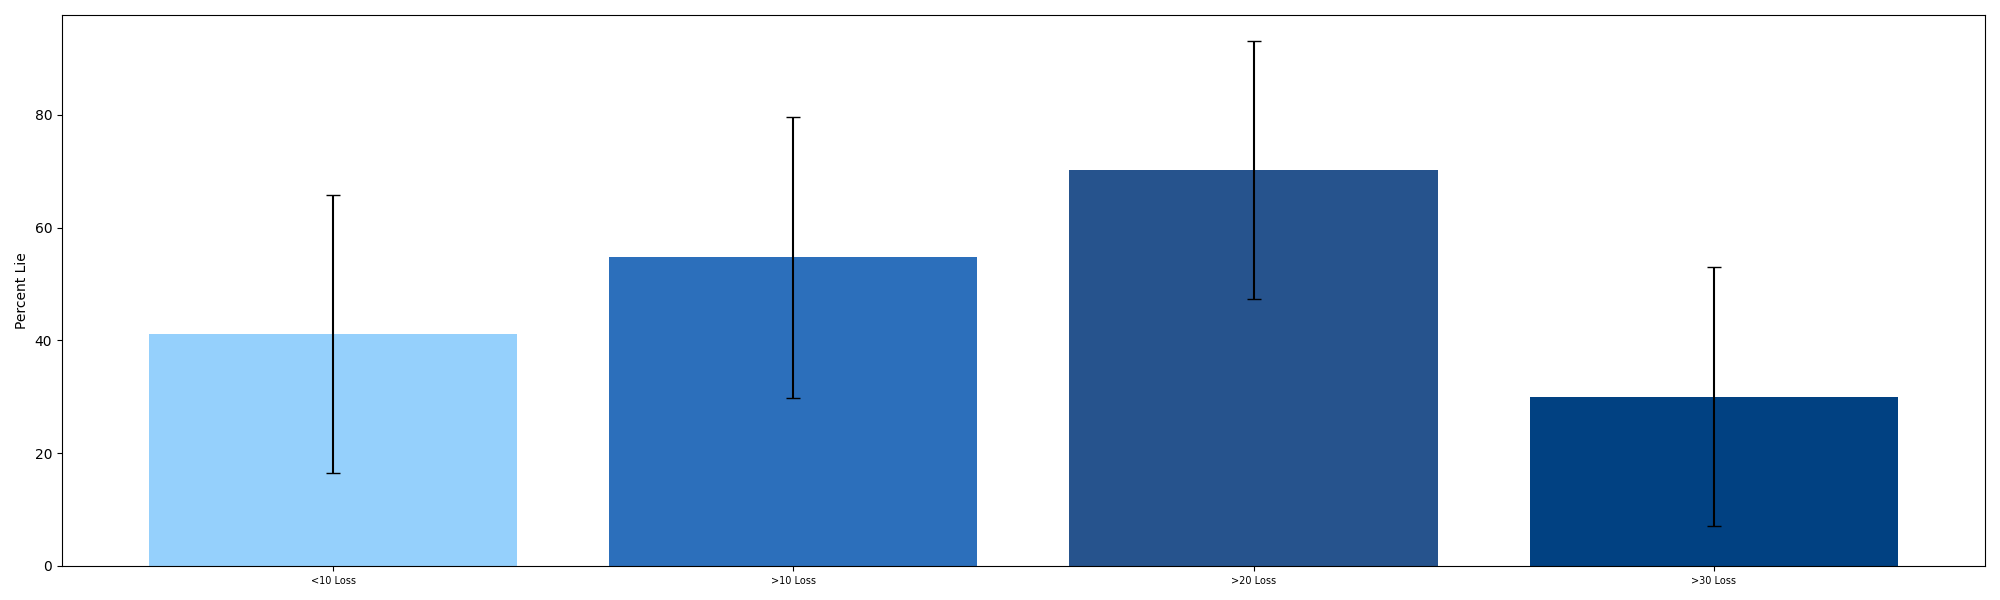
\includegraphics[width=\linewidth]{../plots/RESPONSE/NetLossLie.png}
	\caption{Percentage of senders who chose to lie based on how much the receiver would lose.}
	%	\figurenote{+10 gain represents the proportion who chose to lie for all amounts above 10 and also applies for +20 and +30.}
	\label{fig:NetLossLie}
\end{figure}

Senders were less likely to lie when the losses to the receiver were great. When losses were under 10,  41\% $(N = 1340)$ of senders chose to lie. With losses greater than 10, 55\%  $(N = 1153)$ chose to lie through to losses greater than 20 where the percentage of senders who chose to lie showed a notable increase, to 70\%  $(N = 560)$. When losses to the receiver were larger than thirty the amount of senders was 30\% $(N = 150)$

The difference in lie percentage between trials where losses to the receiver were over 10 and trials where losses to the receiver were under 10 was shown to be significant $\chi^2(1,$ $N=2027) = 45,$ $p<.001$ as well as in trials where losses to the receiver were over and under 30 $\chi^2(1,$ $N=2489) = 4.2,$ $p=.042$.

\subsection{Differences in information gathering strategy}

\subsubsection{By trial condition}

\paragraph{Dwell Time}
Observing Table \ref{tab:CombinedNetDwell}, it can be seen that no differences in dwell are observed across trial conditions that were found to have significant proportional differences in lie outcomes.

\begin{table}[H]
	\centering
	\begin{tabular}{ccccccc}
		\multirow{2}{*}{} & \multicolumn{2}{c}{<10 Gain to Sender} & \multicolumn{2}{c}{>10 Gain to Sender} & \multicolumn{2}{c}{} \\ \cline{2-5}
		& $M$ (ms) &$SD$ (ms) & $M$ (ms) & $SD$ (ms) & $t(2487)$ & $p$ \\ \hline
		SELF LIE & 463 & 441 & 478 & 413 & 0.84 & .798  \\ \hline
		SELF TRUE & 430 & 354 & 408 & 329 & -1.6 & .460  \\ \hline
		OTHER LIE & 555 & 398 & 590 & 448 & 2.0 & .173 \\ \hline
		OTHER TRUTH & 598 & 455 & 611 & 492 & 0.66 & .511 \\ \hline
		\multirow{2}{*}{} & \multicolumn{2}{c}{<30 Gain to Sender} & \multicolumn{2}{c}{>30 Gain to Sender} & \multicolumn{2}{c}{} \\ \cline{2-5}
		& $M$ (ms) &$SD$ (ms) & $M$ (ms) &$SD$ (ms) & $t(2487)$ & $p$ \\ \hline
		SELF LIE & 519 & 486 & 465 & 421 & -1.9 & .235  \\ \hline
		SELF TRUE & 399 & 329 & 422 & 345 & 1.0 & .476  \\ \hline
		OTHER LIE & 610 & 424 & 567 & 422 & -1.5 & .224 \\ \hline
		OTHER TRUTH & 582 & 428 & 607 & 477 & 0.79 & .511 \\ \hline
		\multirow{2}{*}{} & \multicolumn{2}{c}{<10 Loss to Receiver} & \multicolumn{2}{c}{>10 Loss to Receiver} & \multicolumn{2}{c}{} \\ \cline{2-5}
		& $M$ (ms) &$SD$ (ms) & $M$ (ms) & $SD$ (ms) & $t(2491)$ & $p$ \\ \hline
		SELF LIE & 475 & 417 & 478 & 413 & 0.15 & .880  \\ \hline
		SELF TRUE & 418 & 328 & 408 & 329 & -0.71 & .476  \\ \hline
		OTHER LIE & 566 & 410 & 590 & 448 & 1.4 & .224 \\ \hline
		OTHER TRUTH & 594 & 441 & 611 & 492 & 0.92 & .511 \\ \hline
		\multirow{2}{*}{} & \multicolumn{2}{c}{<30 Loss to Receiver} & \multicolumn{2}{c}{>30 Loss to Receiver} & \multicolumn{2}{c}{} \\ \cline{2-5}
		& $M$ (ms) & $SD$ (ms) & $M$ (ms) &$SD$ (ms) & $t(2487)$ & $p$ \\ \hline
		SELF LIE & 471 & 431 & 453 & 379 & 0.51 & .817  \\ \hline
		SELF TRUE & 421 & 345 & 399 & 307 & 0.76 & .476 \\ \hline
		OTHER LIE & 571 & 421 & 571 & 422 & 0.01 & .990 \\ \hline
		OTHER TRUTH & 601 & 470 & 649 & 507 & -1.2 & .511 \\ \hline
	\end{tabular}
	\vspace{0.3cm}
	\caption{Comparison of mean and standard deviation of dwell times for each AOI across different conditions of net gain to Sender and net loss to Receiver. (FDR Corrected)}
	\label{tab:CombinedNetDwell}
\end{table}

\paragraph{Number of Transitions}
The difference in number of transitions proved not to be significant when comparing trials where the net gain to the Sender was above $(M = 5.5\%$, $SD = 4.1\%)$ or below 10 $(M = 5.6\%$, $SD = 4.1\%)$, $t(2487)=-0.5$, $p=.617$.
Similarly the difference in number of transitions showed to be insignificant when comparing trials where the Receiver made a loss of above $(M = 5.5\%$, $SD = 4.1\%)$  or below 10 $(M = 5.6\%$, $SD = 4.1\%)$ from lying, $t(2491)=-0.66$, $p=.617$. Across trials where the net gain to sender was above 30 $(M = 5.1\%$, $SD = 3.6\%)$ and below 30 $(M = 5.6\%$, $SD = 4.2\%)$ there showed to be no significant difference either, $t(2487)=1.9$, $p=.241$. This was also the case for when net loss to the receiver was above 30 $(M = 5.1\%$, $SD = 3.6\%)$ and below 30 $(M = 5.1\%$, $SD = 3.6\%)$, $t(2487)=1.3$, $p=.376$.

\subsubsection{By population clustering}
Hierarchical clustering was used to fit suitable clusters based on the pairwise distance measure calculated between trials using Dynamic Time Warping. Using the Pseudo F statistic and a cluster limit of 20, it was deemed that two clusters represented the best degree of separation and internal cohesiveness. The two clusters, cluster 1 and 2 were made up of 1006 and 1483 trials, respectively.


\paragraph{Dwell Time}
Each of the AOIs showed significant differences across clusters, as seen in Table \ref{tab:DwellTimesPerCluster}.

\begin{table}[H]
	\centering
	\begin{tabular}{|p{1.4cm}|p{1cm}|p{1cm}|p{1cm}|p{1cm}|p{1cm}|p{1cm}|p{1cm}|}
			\hline
			\multirow{2}{*}{} & \multicolumn{2}{c|}{Cluster 1} & \multicolumn{2}{c|}{Cluster 2} & \multicolumn{3}{c|}{Between} \\ \cline{2-8}
			& $M$ (ms) &$SD$ (ms) & $M$ (ms) & $SD$ (ms)  & $t$ & d.o.f. & $p$   \\ \hline
			\small{SELF LIE}& 551 & 392 & 415 & 345 & 8.1 & 2321 & <.001  \\ \hline
			\small{SELF TRUE} & 530 & 309 & 345 & 345& 14 & 2305  &  <.001 \\ \hline
			\small{OTHER LIE} & 633 & 396 &529 & 435 & 6.0 & 2287 &  <.001  \\ \hline
			\small{OTHER TRUTH} & 679 & 452 & 554 & 479 & 6.6 & 2237 &  <.001 \\ \hline
		\end{tabular}
	\vspace{0.3cm}
	\figurenote{d.o.f., in this case, is shorthand for degrees of freedom.}
	\caption{Mean, standard deviation and t tests for the average dwell time of each AOI across participant clusters (FDR corrected).}
	\label{tab:DwellTimesPerCluster}
\end{table}

\begin{figure}[H]
	\centering
	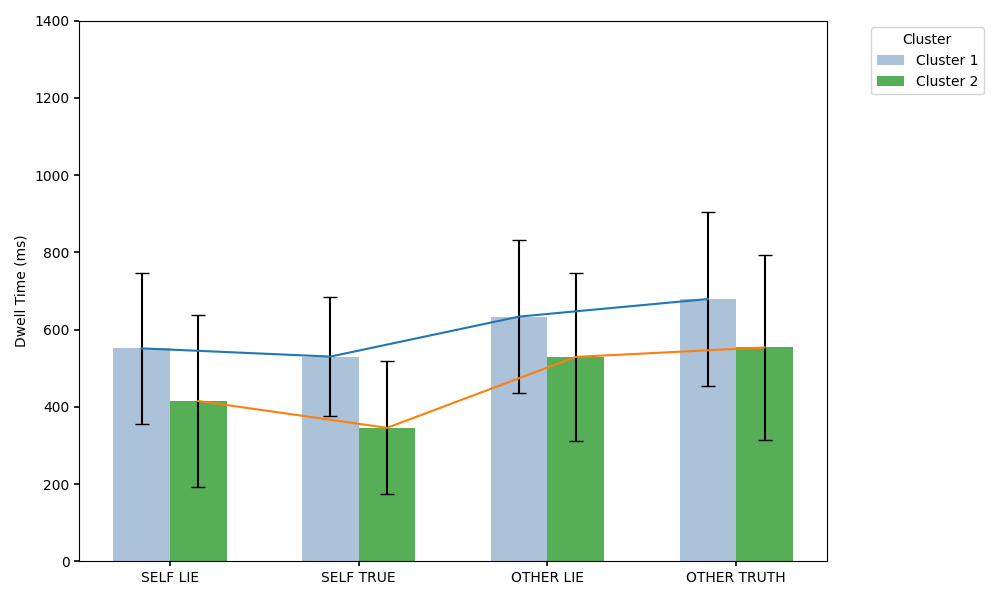
\includegraphics[width=0.75\linewidth]{../plots/ALLTRIAL/DwellTimes.png}
	\caption{Average dwell time across clusters for each AOI.}
	%\figurenote{This is a great figure.}
	\label{fig:DwellTimesPerCluster}
\end{figure}

\paragraph{Number of Transitions}

The average number of transitions across clusters also showed significant differences. With cluster 1 showing a mean level of 8.5 $(SD = 4.1)$ and cluster 2 showing a smaller average of 3.5 $(SD = 2.6)$, $\chi^2(1,$ $N=2027) = 24,$ $p<.001$.

\begin{figure}[H]
	\centering
	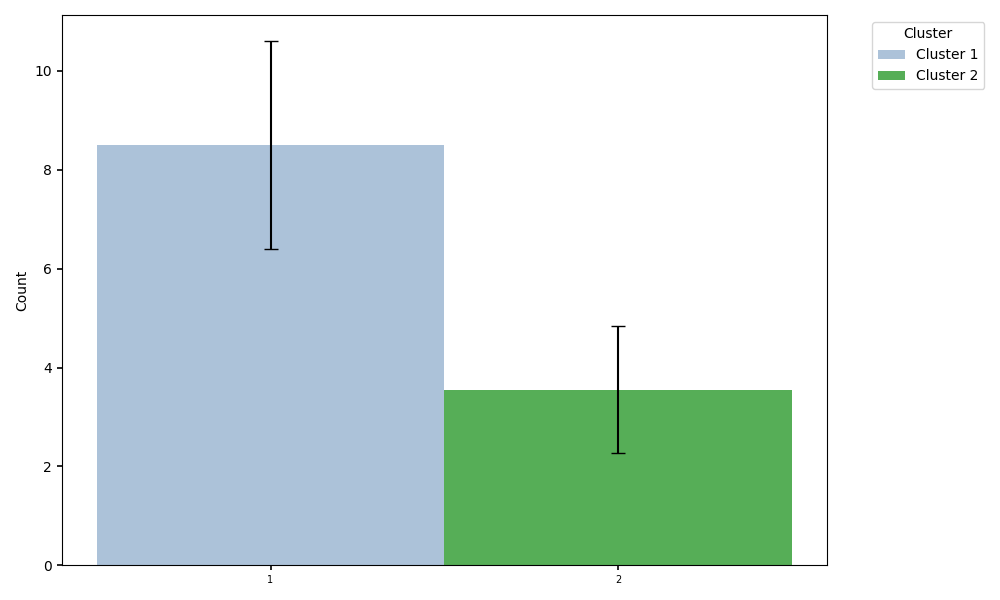
\includegraphics[width=0.75\linewidth]{../plots/ALLTRIAL/NTransitions.png}
	\caption{Average number of transitions calculated per cluster for each participant.}
	%	\figurenote{+10 gain represents the proportion who chose to lie for all amounts above 10 and also applies for +20 and +30.}
	\label{fig:NTransitionsPerCluster}
\end{figure}


\subsection{Information gathering strategy as a predictor of dishonest behaviour}

\subsubsection{Lie proportion by cluster}

There was a significant difference in the proportion of lies across clusters $\chi^2(1,$ $N=2489) = 24,$ $p=<.001$. As observed in Figure \ref{fig:NTrialsByPIDPerCluster}, each participant had trials belonging to both cluster memberships. The quantities, of which fail, to show a linear relationship with lie percentage.

\begin{figure}[H]
	\centering
	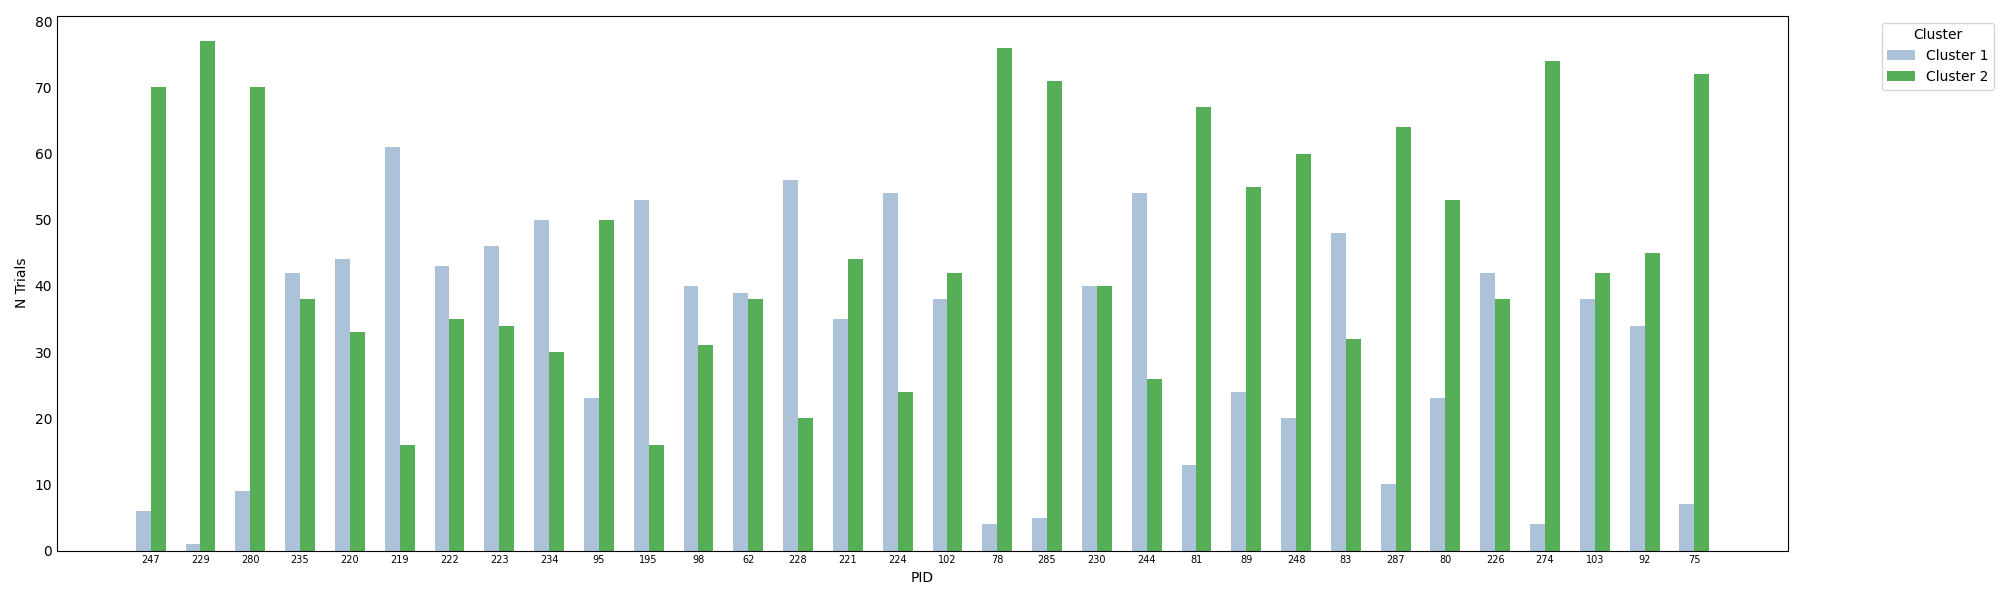
\includegraphics[width=\linewidth]{../plots/ALLTRIAL/NTrialsByPID.png}
	\caption{The number of trials per cluster for each participants. Participants are ordered by the overall proportion of lie chosen in ascending order. Clusters were calculated using hierarchical clustering based on DTW measure.}
	%	\figurenote{+10 gain represents the proportion who chose to lie for all amounts above 10 and also applies for +20 and +30.}
	\label{fig:NTrialsByPIDPerCluster}
\end{figure}

\subsubsection{Modelling the effect of cluster}

A hierarchical logistic regression model was built to assess the effect of cluster by evaluating it alongside task condition variables, amount gained to Sender and loss to the Receiver, as well as whether there was any interaction between the terms. The model used random intercepts across participants to account for the variance observed.

\paragraph{Task Condition} 
In the resulting model, gain to sender showed to have a significant positive effect on lie probability, $\beta = 0.14$, $SE = 0.01$, $p = < .001$. Each unit of increase in self-gain resulted in the odds of lying increasing by approximately 15.5\% $(OR=1.15)$. Loss to receiver showed to have a significant negative effect on lie probability $\beta = -0.09$, $SE = 0.01$, $p = < .001$ with the odds of lying decreasing by approximately 8.5\% for each unit of increased loss $(OR=0.91)$. 
\paragraph{Cluster} 
Cluster showed to, also, have a significant effect on lie probability $\beta = 0.58$, $SE = 0.20$, $p = < .001$. Cluster 2 participants were 78.2\% more likely to lie than Cluster 1 participants $(OR=1.78)$.
\paragraph{Interaction}
The interaction between gain to Sender and cluster was shown to be significant, $\beta = -0.04$, $SE = 0.01$, $p = < .001$. This suggests that the effect of the amount gained by the Sender on the likelihood of lying was weaker in Cluster 2, where each unit increase in amount was associated with a decrease in the odds of lying by approximately 4.4\% $(OR=0.96)$. In Figure \ref{fig:InteractionEffects}, it can be seen that the probability of a lie was lower for Cluster 1 than it was for Cluster 2, however, at very high values Cluster 1 showed the greater likelihood. The interaction between amount lost by Receiver and cluster membership was found not to be significant, $\beta = -0.02$, $SE = 0.01$, $p = .115$.


\begin{figure}[H]
	\centering
	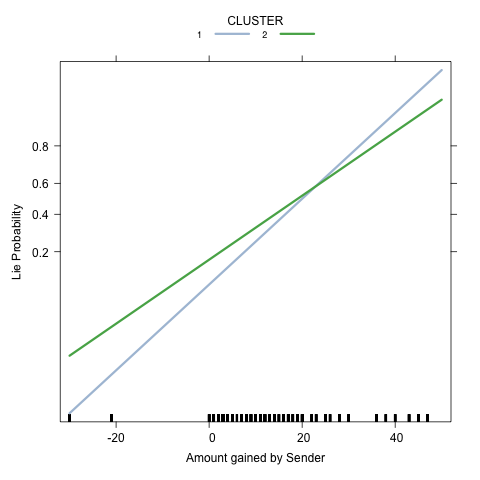
\includegraphics[width=0.75\linewidth]{../plots/R_selfgain/effects.png}
	\caption{The probability that lie will be the response as amount gained by the Sender increases for both clusters.}
	%	\figurenote{+10 gain represents the proportion who chose to lie for all amounts above 10 and also applies for +20 and +30.}
	\label{fig:InteractionEffects}
\end{figure}

\paragraph{Model Diagnostics}

\begin{figure}[H]
	\centering
	
	% First subfigure
	\begin{subfigure}[b]{0.45\textwidth}
		\centering
		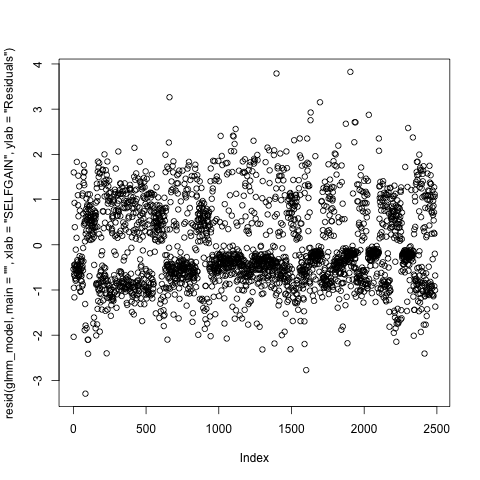
\includegraphics[width=\textwidth]{../plots/R/residuals}
%		\caption{Caption for the first image (Residuals).}
		\label{fig:residuals}
	\end{subfigure}
	\hfill
	% Second subfigure
	\begin{subfigure}[b]{0.45\textwidth}
		\centering
		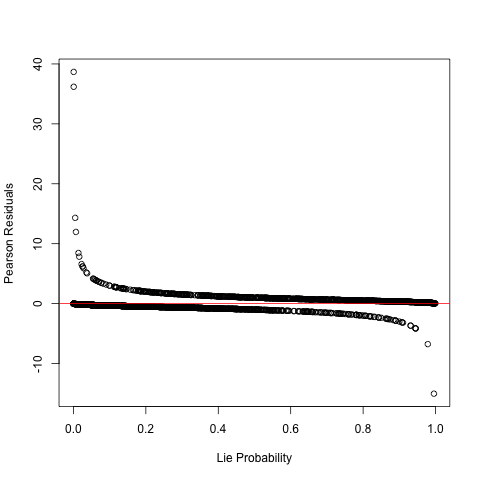
\includegraphics[width=\textwidth]{../plots/R/pearson_residuals_vs_fitted}
%		\caption{Caption for the second image (Pearson Residuals vs Fitted).}
		\label{fig:pearsonresidualsvsfitted}
	\end{subfigure}
	
	\caption{(left) Residuals plot with index of observation on x-axis (right) Pearson residuals plot}
	\label{fig:Residuals}
\end{figure}

Looking at the plots in Figure \ref{fig:Residuals} there shows to be some noticeable outliers. The Pearson residuals plot reflects attributes associated with heteroscedasticity around probabilities that represent almost certainty. Similarly the Q-Q plot in \ref{fig:qqline} shows outliers at the upper and lower most quantiles. The model shows a better fit above the central tendency, suggesting that it is better at predicting lies than truths.

\begin{figure}[H]
	\centering
	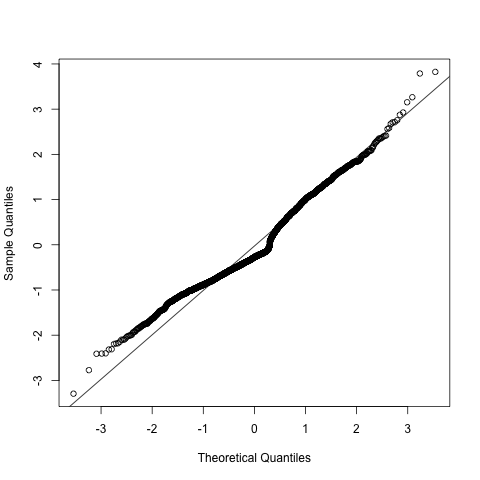
\includegraphics[width=0.5\linewidth]{../plots/R/qqline}
	\caption{Q-Q plot mapping the theoretical normal distribution of quantities on to the sample ones}
	\label{fig:qqline}
\end{figure}

\section{Discussion}

% - Understand whether perceived monetary outcomes to self and another have an affect on the way we gather information
% - Determine if information gathering strategy in social decision making reflects an individual preference
% - Ask whether information gathering strategy can be used a predictor in social decision making

%Stuff to talk about in the conclusion
% answering the aims
% the viability of the model
% limitations
% - lack of data

% eye tracking, implicit cognition and neuro data
% bounded rationality


The results show some differences in information strategy. Differences in strategy were found not to alter based on perceived monetary gains and lie percentage but showed significant differences when comparing trials at the individual level, condition-agnostic. The set of valid trials were successfully clustered in to two memberships using hierarchical clustering. The clusters showed to have significant differences in terms of their attributes. Cluster 1 was characterised with a larger number of transitions and longer dwell times for each of the four AOIs than that of cluster 2. Cluster 2 had dwell times that were shorter and a average number of transitions that was significantly less. The differences between the clusters shows to be largely uniform across all four AOIs (see Figure \ref{fig:DwellTimesPerCluster}) suggesting that strategical differences could not be distinguished with respect to any particular AOI. 

The difference in strategical attributes found between cluster 1 and cluster 2 largely suggest that trials in cluster 1 were subject to a more patient and considered approach than that of the trials in cluster 2. Cluster 1 shows greater levels of adjacency where cluster 2 trials show significantly reduced levels. With a mean number of transitions of 3.5 for cluster 2, the trials in this cluster show a characterisation of possessing the minimum level of adjacency needed to draw comparison between informational attributes in the trial provided there is a at least one occurrence for each with no absences. It can therefore be inferred that the trials in cluster 2 have qualities that are closer in line with sequential search. Where each occurrence of an AOI is seen at an increasing effort cost to the participant and subject to termination when a particular threshhold is achieved; much in the same vein as the satisficing heuristic laid out by Simon. The trials in cluster 1 show a far greater number of transitions between the four AOIs (as seen in Figure \ref{fig:NTransitionsPerCluster}) suggesting effort cost was less of a limiting factor. The increased dwell times for cluster 1 suggesting time spent looking was too.

Each cluster possessed a higher probability of outputting a lie at different levels of amount earned. As seen in work by Gneezy and in \ref{fig:} the likelihood of lying is decreased at lower values because a person's utility ie. it's desire to maximise gain is reduced. All Both clusters possessed lesser likelihood of a lie choice at lower values, suggesting participants were willing to forgo minimal returns in order to exhibit altruistic tendencies




Each participant were shown to have a proportion of their trials belonging to either membership, as per \ref{fig:NTrialsByPIDPerCluster}. 


The Figure , represents the breakdown of the number of each trials for each participant, ordered by percentage lies. As can be seen



% Results/Findings which includes: analyses performed, reporting of analyses, use of graphs/tables/diagrams, organization and structure, and clarity
% analyses performed:
% RT, Dwell Times
% Gains
% DTW 

%\subsection{Participant Analysis}
%
%An analysis was performed on the distance data extracted from the time series analysis at the participant level. The results of which, are taken from averaging the distance between all of the trials of a single participant against another. Through hierarchical clustering and silhouette analysis, the participants were separated in to two clusters.
%
%\begin{figure}[H]
%	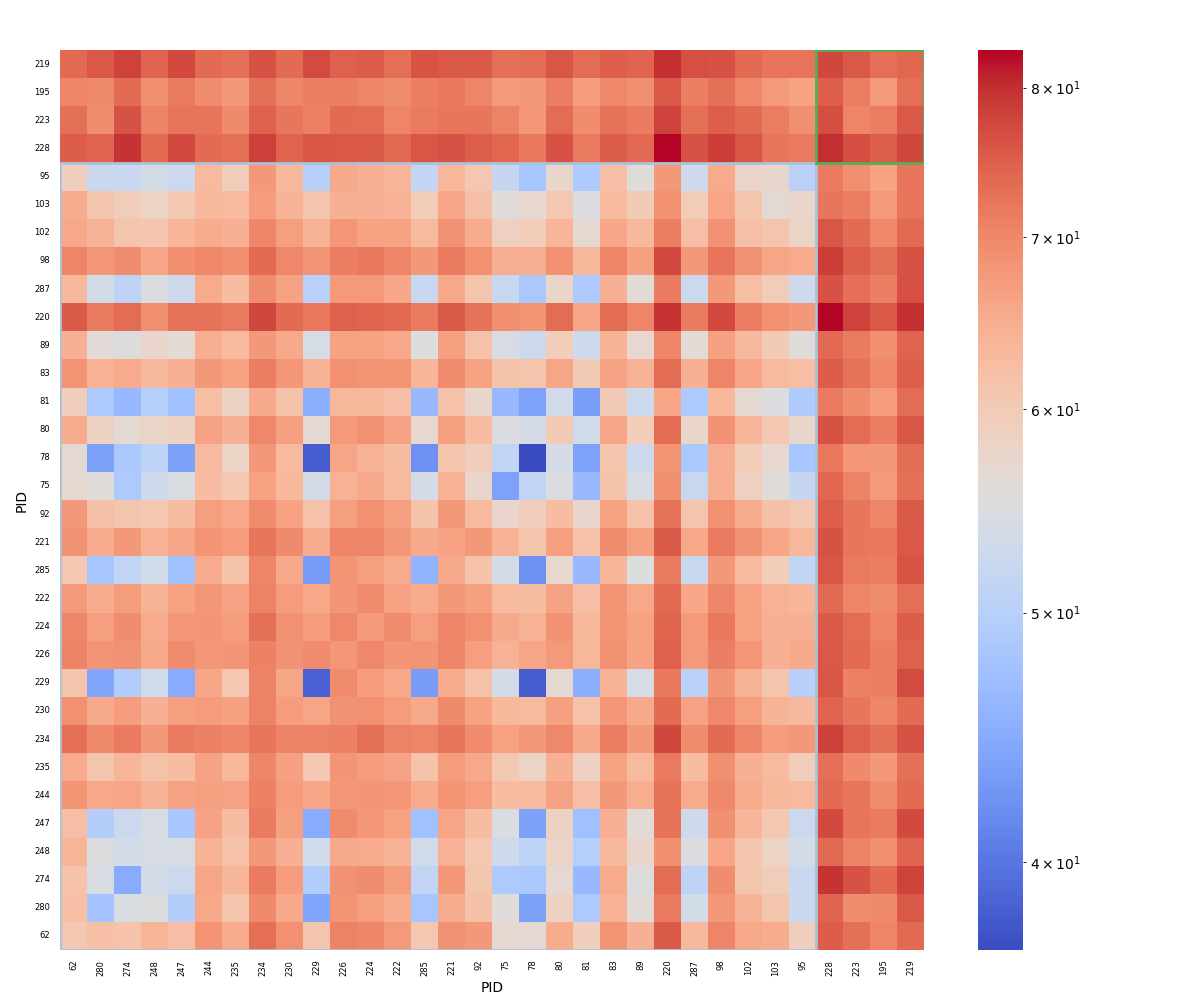
\includegraphics[width=\linewidth]{../plots/PID/DistanceMatrix.png}
%	\caption{Matrix showing the similarity between participants taken from their mean euclidean distance measure shared with one and another. The matrix is sorted by proximity with the two clusters of participants outlined.}
%	%	\figurenote{+10 gain represents the proportion who chose to lie for all amounts above 10 and also applies for +20 and +30.}
%	\label{fig:DistanceMatrix}
%\end{figure}
%
%\subsubsection{Lie Percentage}
%
%\begin{figure}[H]
%	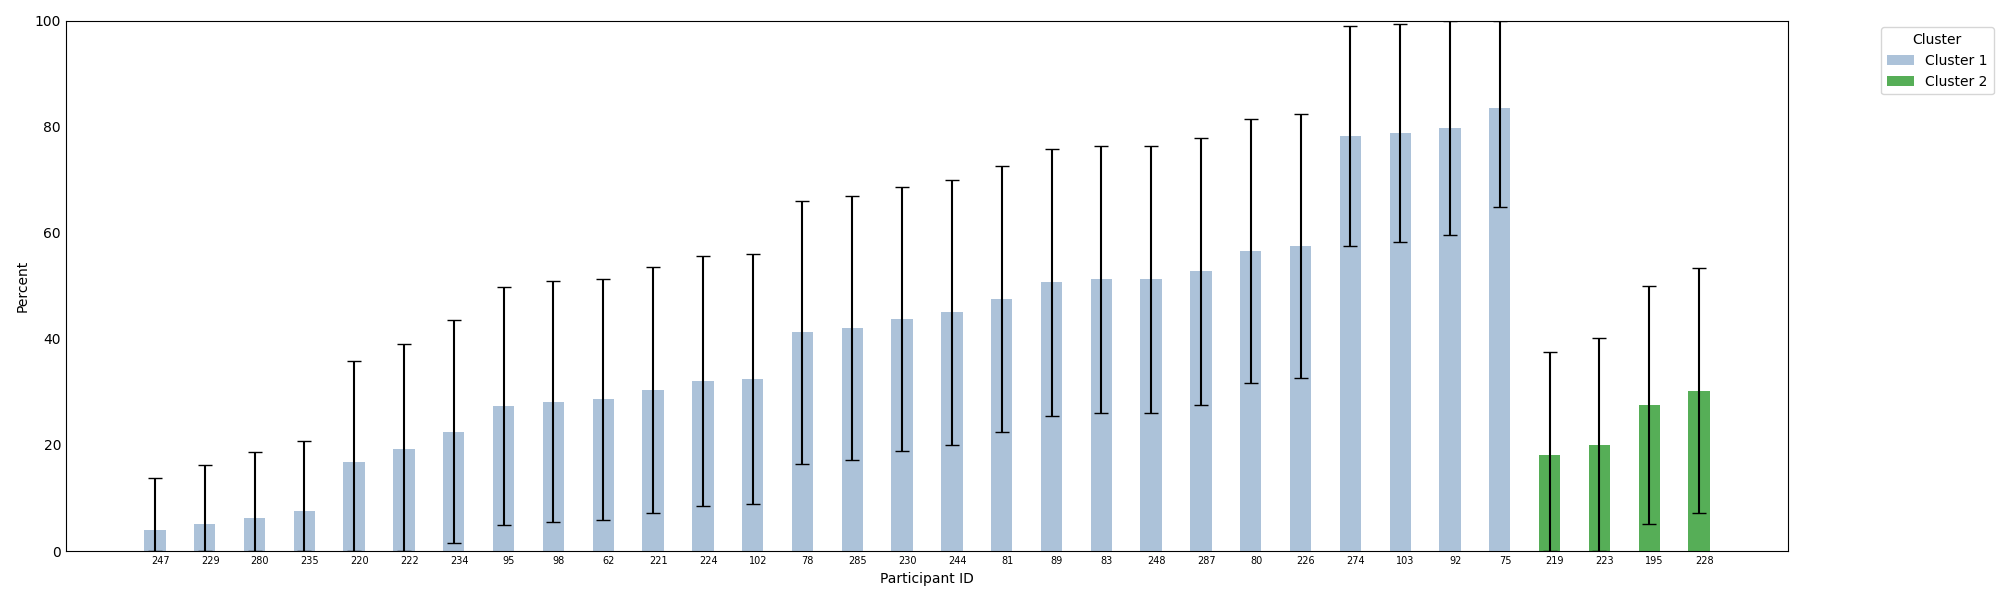
\includegraphics[width=\linewidth]{../plots/PID/PercentLiesByPID.png}
%	\caption{Participants separated by hierarchical distance clustering and ordered by percentage lies.}
%	%	\figurenote{+10 gain represents the proportion who chose to lie for all amounts above 10 and also applies for +20 and +30.}
%	\label{fig:PercentLiesByPIDCluster}
%\end{figure}
%
%Using pairwise t-tests and calculating the mean statistic across clusters, it was deemed that the two clusters and their participant memberships showed to have a difference in lie percentage that was not significant $t(30)=1.4$, $p=.181$ (FDR corrected). Cluster 1 had a mean lie percentage of 40\% $(SD = 49\%)$ and cluster 2 had a mean of 23\% $(SD = 42\%)$. 
%
%\subsubsection{Dwell Time}
%
% \begin{figure}[H]
% 	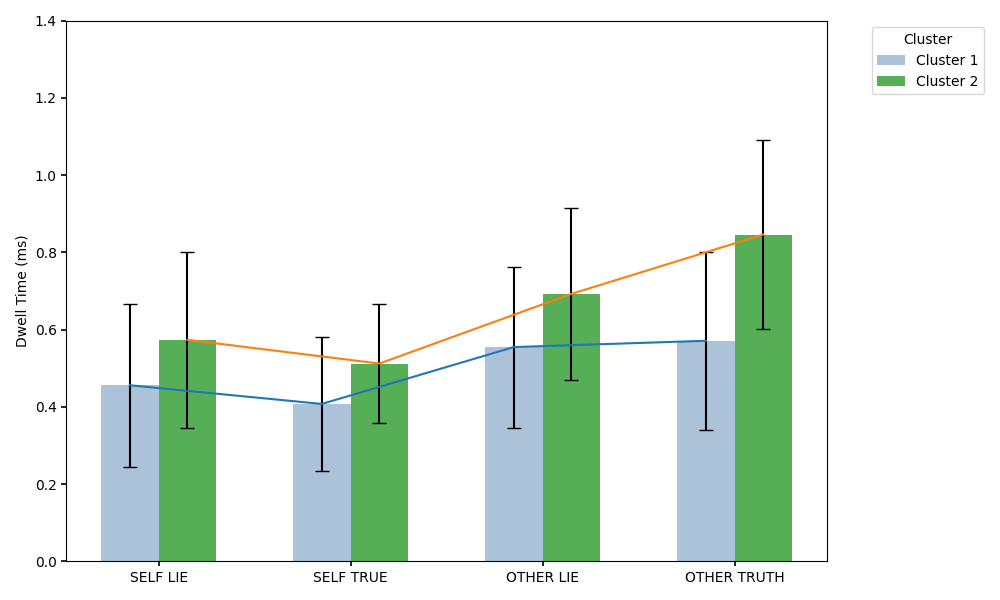
\includegraphics[width=\linewidth]{../plots/PID/DwellTimes.png}
% 	\caption{Measures of average dwell time across participant clusters segmented by hierarchical distance clustering.}
% 	%	\figurenote{+10 gain represents the proportion who chose to lie for all amounts above 10 and also applies for +20 and +30.}
% 	\label{fig:DwellTimesByPIDCluster}
% \end{figure}
%
%\begin{table}[H]
%	\centering
%	\begin{tabular}{|p{1.4cm}|p{1cm}|p{1cm}|p{1cm}|p{1cm}|p{1cm}|p{1cm}|p{1cm}|p{1cm}|p{1cm}|p{1cm}|}
%		\hline
%		\multirow{2}{*}{} & \multicolumn{4}{c|}{Cluster 1} & \multicolumn{4}{c|}{Cluster 2} & \multicolumn{2}{c|}{Between} \\ \cline{2-11}
%		& $M$ (ms) &$SD$ (ms) & $t(378)$ & $p$ & $M$ (ms) & $SD$ (ms) & $t(112)$ & $p$ & $t(6)$ & $p$ \\ \hline
%		\small{SELF LIE}& 456 & 423 & 0.79 & .182 & 573 & 455 & -1.6 & .169 & 0.68 & .187  \\ \hline
%		\small{SELF TRUE} & 407 & 346 & 0.58 & .138 & 512 & 307 & -1.3 & .293 & 0.40 & .191  \\ \hline
%		\small{OTHER LIE} & 555 & 417 & -0.29 & .258 & 693 & 444 & -2.9 & .103 & -0.60 & .231 \\ \hline
%		\small{OTHER TRUTH} & 571 & 461 & -0.67 & .213 & 846 & 487 & -2.7 & .064 & -0.98 & .138 \\ \hline
%	\end{tabular}
%	\vspace{0.3cm}
%	\caption{Mean,. standard deviation and t tests for the average dwell time of each AOI across participant clusters. (FDR corrected)}
%	\label{tab:NetLossDwellByPID}
%\end{table}
%
%
%In Table \ref{tab:NetLossDwellByPID}, average dwell times across the four AOIs show no significant differences when compared between and within clusters of participant membership.
%
%\subsubsection{Number of Transitions}
%
% \begin{figure}[H]
%	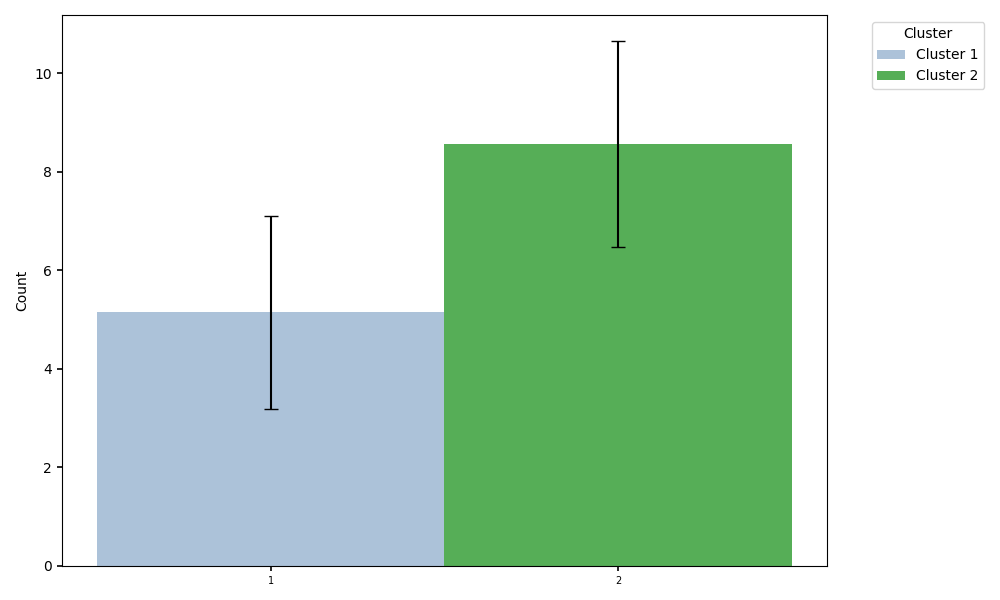
\includegraphics[width=\linewidth]{../plots/PID/NTransitions.png}
%	\caption{Average number of transitions between clusters of participants determined from hierarchical clustering.}
%	%	\figurenote{+10 gain represents the proportion who chose to lie for all amounts above 10 and also applies for +20 and +30.}
%	\label{fig:NTransitionsByPIDCluster}
%\end{figure}
%
%The number of transitions averaged by the participants in Cluster 1 $(M = 5.1$, $SD = 3.9)$, showed to be significantly different to that of the participants in Cluster 2 $(M = 8.6\%$, $SD = 4.2\%)$, $t(112)=0.60$, $p=.070$. Comparatively, there was no significant difference in number of transitions within  Cluster 1 $t(378)=0.44$, $p=.0604$ but Cluster 2 $t(6)=3.5$, $p=.026$ there was found to be a significant difference (FDR corrected).
%
%\subsection{Cross Analysis}
%
%\subsubsection{Lie Percentage}
%
% \begin{figure}[H]
%	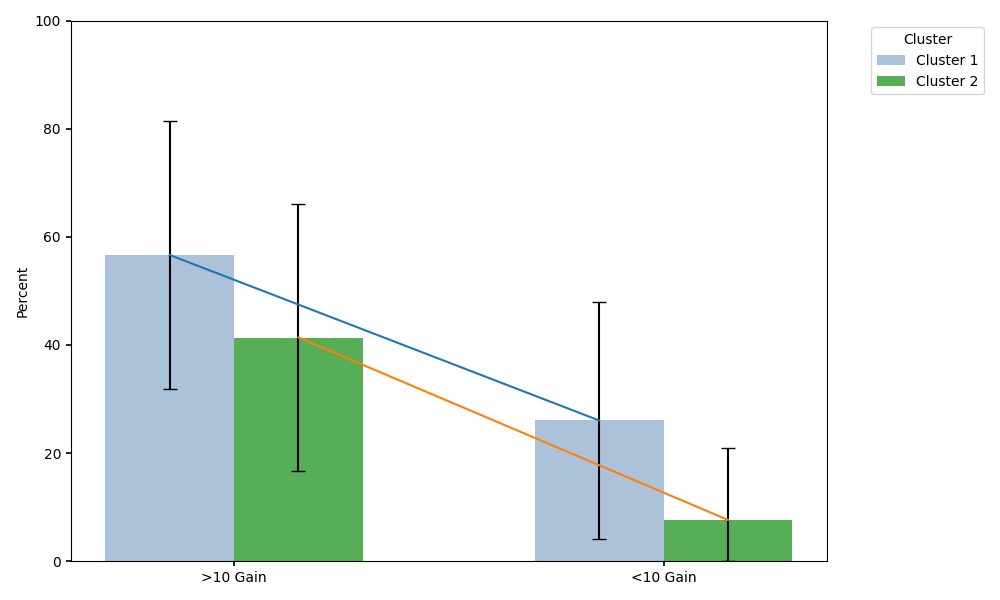
\includegraphics[width=\linewidth]{../plots/GainCluster/PercentLies.png}
%	\caption{Average lie percentage for each cluster of participants across trial conditions dependent on net gain to sender.}
%	%	\figurenote{+10 gain represents the proportion who chose to lie for all amounts above 10 and also applies for +20 and +30.}
%	\label{fig:PercentLiesPerGainByPIDCluster}
%\end{figure}
%
%\begin{table}[H]
%	\centering
%	\begin{tabular}{|c|p{1.5cm}|p{2cm}|p{1.5cm}|p{2cm}|p{2cm}|p{1.5cm}|}
%		\hline
%		\multirow{2}{*}{} & \multicolumn{2}{c|}{<10 Gain to Sender} & \multicolumn{2}{c|}{>10 Gain to Sender} & \multicolumn{2}{c|}{T-test result} \\ \cline{2-7}
%		& $M$ (\%) &$SD$ (\%) & $M$ (\%) & $SD$ (\%) & $t(66)$ & $p$ \\ \hline
%		Cluster 1& 20 & 40 & 56 & 49 & -0.26 & .793  \\ \hline
%		Cluster 2 & 34 & 47 & 52 & 50 & -0.74 & .460  \\ \hline
%	\end{tabular}
%	\vspace{0.3cm}
%	\caption{Comparison of mean and standard deviation of average percent lie for each cluster across trial conditions (FDR Corrected)}
%	\label{tab:PercentLiesPerGainByPIDCluster}
%\end{table}
%
%
%
%\subsubsection{Dwell Time}
%
% \begin{figure}[H]
%	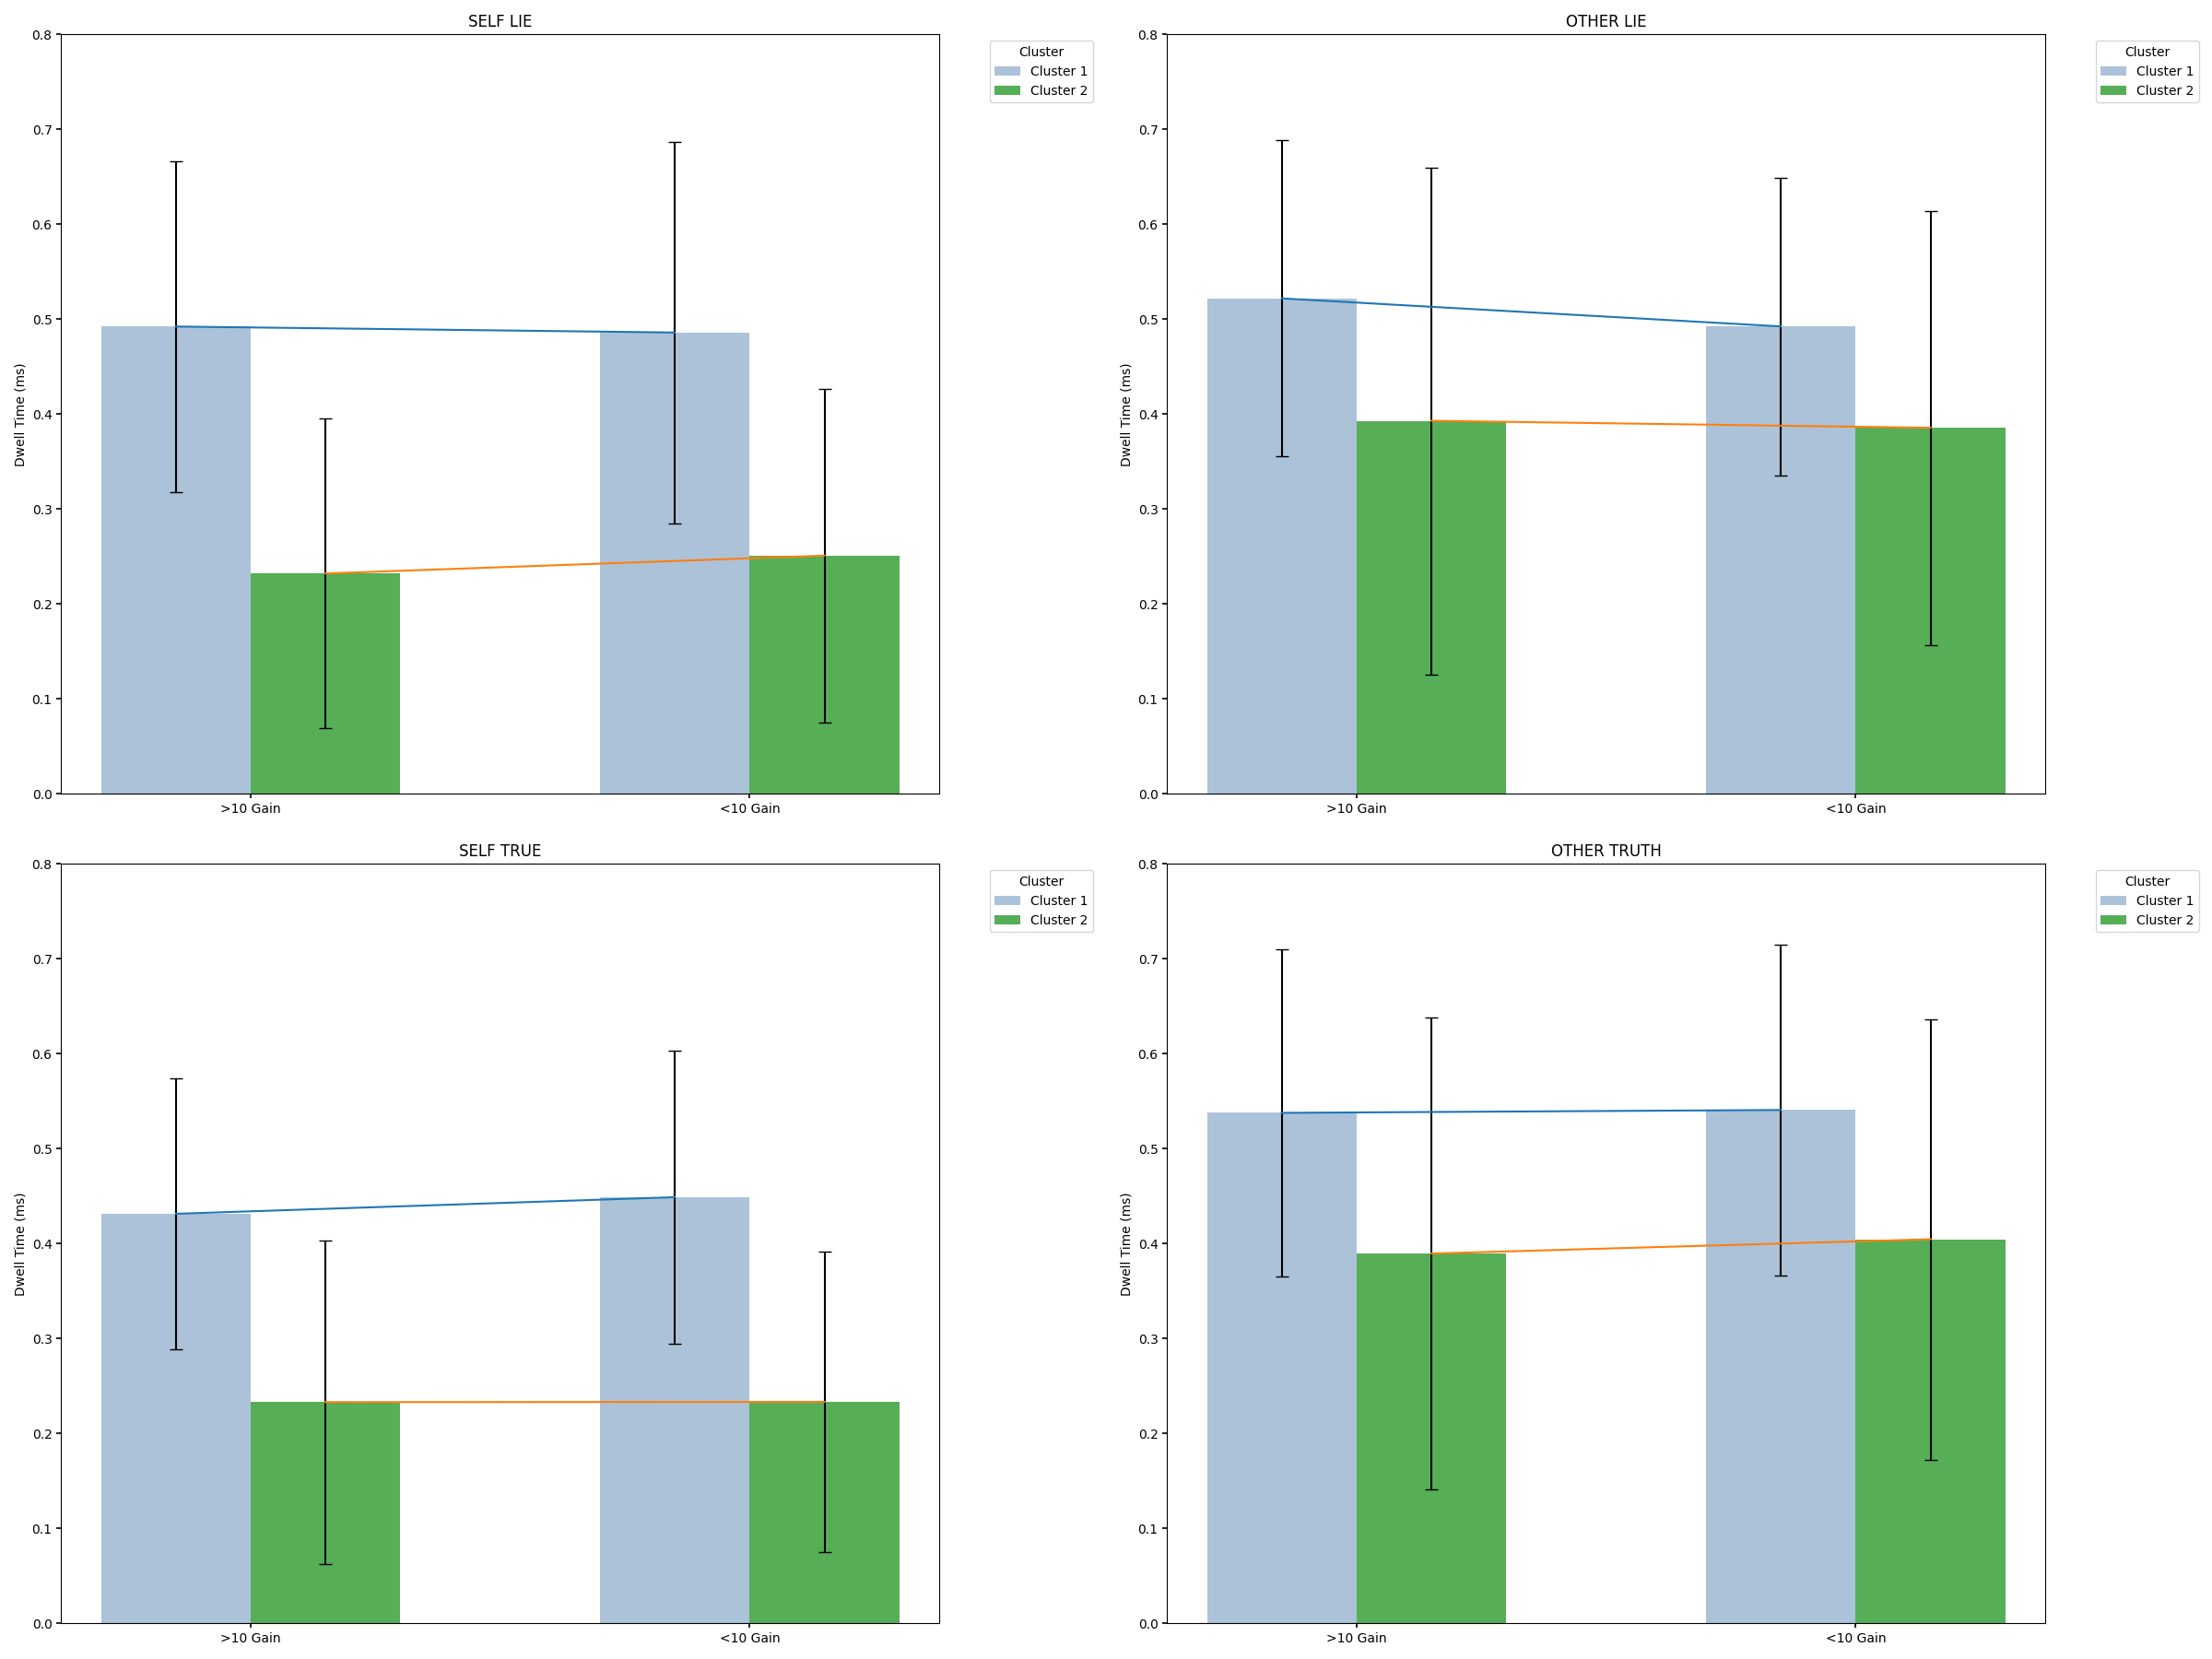
\includegraphics[width=\linewidth]{figures/GainClusterTiles.png}
%	\caption{Measures of average dwell time across participant clusters segmented by hierarchical distance clustering.}
%	\label{fig:DwellTimesPerGainByPIDCluster}
%\end{figure}
%
%\begin{table}[H]
%	\centering
%	\begin{tabular}{|p{3.2cm}|p{0.7cm}|p{0.7cm}|p{0.7cm}|p{0.7cm}|p{0.9cm}|p{0.7cm}|p{0.7cm}|p{0.7cm}|p{0.8cm}|p{0.7cm}|}
%		\hline
%		\multirow{2}{*}{} & \multicolumn{4}{c|}{Gain to Sender < 10} & \multicolumn{4}{c|}{Gain to Sender > 10} & \multicolumn{2}{c|}{} \\ \cline{2-11}
%		\multirow{2}{*}{} & \multicolumn{2}{c|}{Cluster 1} & \multicolumn{2}{c|}{Cluster 2} & \multicolumn{2}{c|}{Cluster 1} & \multicolumn{2}{c|}{Cluster 2} & \multicolumn{2}{c|}{T-test result} \\ \cline{2-11}
%		& $M$ (ms) &$SD$ (ms) & $M$ (ms) & $SD$ (ms) & $M$ (ms) &$SD$ (ms) & $M$ (ms) & $SD$ (ms) & $t(34)$ & $p$ \\ \hline
%		SELF LIE& 0.49 & 0.38 & 0.24 & 0.34 & 0.49 & 0.38 & 0.24 & 0.34 & 1.9 & .126  \\ \hline
%		SELF TRUE & 0.44 & 0.30 & 0.23 & 0.33 & 0.49 & 0.38 & 0.24 & 0.34 & 1.5 & .081  \\ \hline
%		OTHER LIE & 0.51 & 0.32 & 0.39 & 0.49 & 0.49 & 0.38 & 0.24 & 0.34 & 0.19 & .211 \\ \hline
%		OTHER TRUTH & 0.54 & 0.35 & 0.40 & 0.48 & 0.49 & 0.38 & 0.24 & 0.34 & -0.15 & .184 \\ \hline
%	\end{tabular}
%	\vspace{0.3cm}
%	\caption{Mean and standard deviation of the dwell time of each AOI across participant clusters. }
%	\label{tab:NetGainDwellByPIDCluster}
%\end{table}
%
%
%\subsubsection{Number of Transitions}
%
% \begin{figure}[H]
%	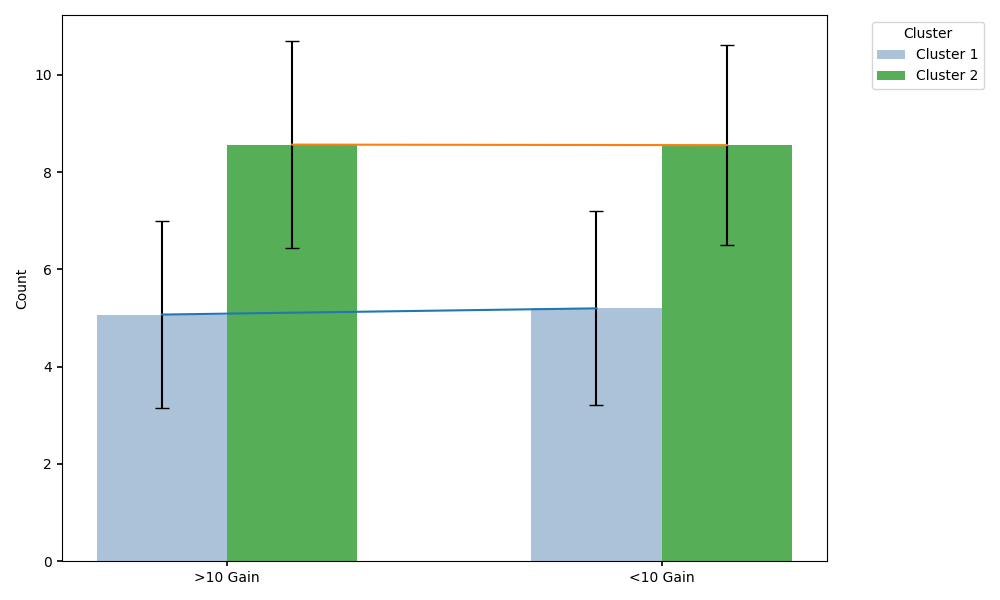
\includegraphics[width=\linewidth]{../plots/GainCluster/NTransitions.png}
%	\caption{Measures of average dwell time across participant clusters segmented by hierarchical distance clustering.}
%	%	\figurenote{+10 gain represents the proportion who chose to lie for all amounts above 10 and also applies for +20 and +30.}
%	\label{fig:NTransitionPerGainByPIDCluster}
%\end{figure}





%The analyses are presented in this section. These analyses may be quantitative or qualitative. Feel free to use as many graphs, tables and diagrams as you think necessary for presenting the analyses clearly.  Do not comment on the meaning of the results here. Extrapolating from your results will happen in your Discussion section



% Discussion which includes: summary of results/findings, understanding of results/findings, critical perspective and insight, indication of future research, organization and structure, and clarity

%In this section, you will summarise your project, expand upon your results, offer insights into strength ms and limitations of your study and/or future directions.

\printbibliography

% References which includes correct use of APA/BPS conventions

\appendix

%This section should contain details which are not essential to understanding the essence of the report. Lists of stimuli, tables of raw data, details of statistical analyses should be included here. The section must be neatly presented and clearly labelled. If you have a very large amount of data, such as might arise in qualitative studies you should consult with your supervisor about what should be included and how.

\end{document}